% Options for packages loaded elsewhere
\PassOptionsToPackage{unicode}{hyperref}
\PassOptionsToPackage{hyphens}{url}
%
\documentclass[
]{article}
\title{Accurate inference of microbial differential abundance from taxonomically-biased microbiome measurements}
\author{Michael R. McLaren\footnote{North Carolina State University; send correspondence to \href{mailto:m.mclaren42@gmail.com}{\nolinkurl{m.mclaren42@gmail.com}}} \and Karen G. Lloyd\footnote{University of Tennessee} \and Benjamin J. Callahan\footnote{North Carolina State University}}
\date{2021-09-15}

\usepackage{amsmath,amssymb}
\usepackage{lmodern}
\usepackage{iftex}
\ifPDFTeX
  \usepackage[T1]{fontenc}
  \usepackage[utf8]{inputenc}
  \usepackage{textcomp} % provide euro and other symbols
\else % if luatex or xetex
  \usepackage{unicode-math}
  \defaultfontfeatures{Scale=MatchLowercase}
  \defaultfontfeatures[\rmfamily]{Ligatures=TeX,Scale=1}
\fi
% Use upquote if available, for straight quotes in verbatim environments
\IfFileExists{upquote.sty}{\usepackage{upquote}}{}
\IfFileExists{microtype.sty}{% use microtype if available
  \usepackage[]{microtype}
  \UseMicrotypeSet[protrusion]{basicmath} % disable protrusion for tt fonts
}{}
\makeatletter
\@ifundefined{KOMAClassName}{% if non-KOMA class
  \IfFileExists{parskip.sty}{%
    \usepackage{parskip}
  }{% else
    \setlength{\parindent}{0pt}
    \setlength{\parskip}{6pt plus 2pt minus 1pt}}
}{% if KOMA class
  \KOMAoptions{parskip=half}}
\makeatother
\usepackage{xcolor}
\IfFileExists{xurl.sty}{\usepackage{xurl}}{} % add URL line breaks if available
\IfFileExists{bookmark.sty}{\usepackage{bookmark}}{\usepackage{hyperref}}
\hypersetup{
  pdftitle={Accurate inference of microbial differential abundance from taxonomically-biased microbiome measurements},
  pdfauthor={Michael R. McLaren; Karen G. Lloyd; Benjamin J. Callahan},
  hidelinks,
  pdfcreator={LaTeX via pandoc}}
\urlstyle{same} % disable monospaced font for URLs
\usepackage[top=1in,bottom=1in,left=1.5in,right=1.5in]{geometry}
\usepackage{longtable,booktabs,array}
\usepackage{calc} % for calculating minipage widths
% Correct order of tables after \paragraph or \subparagraph
\usepackage{etoolbox}
\makeatletter
\patchcmd\longtable{\par}{\if@noskipsec\mbox{}\fi\par}{}{}
\makeatother
% Allow footnotes in longtable head/foot
\IfFileExists{footnotehyper.sty}{\usepackage{footnotehyper}}{\usepackage{footnote}}
\makesavenoteenv{longtable}
\usepackage{graphicx}
\makeatletter
\def\maxwidth{\ifdim\Gin@nat@width>\linewidth\linewidth\else\Gin@nat@width\fi}
\def\maxheight{\ifdim\Gin@nat@height>\textheight\textheight\else\Gin@nat@height\fi}
\makeatother
% Scale images if necessary, so that they will not overflow the page
% margins by default, and it is still possible to overwrite the defaults
% using explicit options in \includegraphics[width, height, ...]{}
\setkeys{Gin}{width=\maxwidth,height=\maxheight,keepaspectratio}
% Set default figure placement to htbp
\makeatletter
\def\fps@figure{htbp}
\makeatother
\setlength{\emergencystretch}{3em} % prevent overfull lines
\providecommand{\tightlist}{%
  \setlength{\itemsep}{0pt}\setlength{\parskip}{0pt}}
\setcounter{secnumdepth}{5}
\newlength{\cslhangindent}
\setlength{\cslhangindent}{1.5em}
\newlength{\csllabelwidth}
\setlength{\csllabelwidth}{3em}
\newlength{\cslentryspacingunit} % times entry-spacing
\setlength{\cslentryspacingunit}{\parskip}
\newenvironment{CSLReferences}[2] % #1 hanging-ident, #2 entry spacing
 {% don't indent paragraphs
  \setlength{\parindent}{0pt}
  % turn on hanging indent if param 1 is 1
  \ifodd #1
  \let\oldpar\par
  \def\par{\hangindent=\cslhangindent\oldpar}
  \fi
  % set entry spacing
  \setlength{\parskip}{#2\cslentryspacingunit}
 }%
 {}
\usepackage{calc}
\newcommand{\CSLBlock}[1]{#1\hfill\break}
\newcommand{\CSLLeftMargin}[1]{\parbox[t]{\csllabelwidth}{#1}}
\newcommand{\CSLRightInline}[1]{\parbox[t]{\linewidth - \csllabelwidth}{#1}\break}
\newcommand{\CSLIndent}[1]{\hspace{\cslhangindent}#1}
\usepackage{cancel}

% Define note environment based on example from https://bookdown.org/yihui/rmarkdown-cookbook/custom-blocks.html
\usepackage{color}
\usepackage{framed}
\setlength{\fboxsep}{.8em}
\newenvironment{rmdnote}{
  \definecolor{shadecolor}{RGB}{248,248,248}
  \begin{shaded}}
 {\end{shaded}}
\ifLuaTeX
  \usepackage{selnolig}  % disable illegal ligatures
\fi

\usepackage{amsthm}
\newtheorem{theorem}{Theorem}[section]
\newtheorem{lemma}{Lemma}[section]
\newtheorem{corollary}{Corollary}[section]
\newtheorem{proposition}{Proposition}[section]
\newtheorem{conjecture}{Conjecture}[section]
\theoremstyle{definition}
\newtheorem{definition}{Definition}[section]
\theoremstyle{definition}
\newtheorem{example}{Example}[section]
\theoremstyle{definition}
\newtheorem{exercise}{Exercise}[section]
\theoremstyle{definition}
\newtheorem{hypothesis}{Hypothesis}[section]
\theoremstyle{remark}
\newtheorem*{remark}{Remark}
\newtheorem*{solution}{Solution}
\begin{document}
\maketitle

{
\setcounter{tocdepth}{2}
\tableofcontents
}
\hypertarget{preface}{%
\section*{Preface}\label{preface}}
\addcontentsline{toc}{section}{Preface}

\emph{This manuscript was rendered from commit 6932587bd1ea9c56638c0ebe3ff7885b79b84e8c.}

\leavevmode\vadjust pre{\hypertarget{preface-warning}{}}%
\textbf{This in-progress manuscript is not intended for general scientific use.}
It is incomplete, has not been carefully reviewed, and may contain mistakes or other inaccuracies.
Please post comments or questions on the \href{https://github.com/mikemc/differential-abundance-theory/issues}{GitHub Issues page} or \href{m.mclaren42@gmail.com}{email Mike}.

This manuscript addresses the effect that the taxonomic bias inherent in microbiome measurement has on microbial differential-abundance analysis.
We describe the basic problem posed by taxonomic bias for measuring changes in the abundance of particular taxa across conditions and describe new strategies for mitigating the errors it induces.
Analyses of both relative and absolute abundances are considered.
In its current form, the manuscript sits somewhere between a standard scientific article and a monograph;
it consists of an article followed by a series of appendices which together give a comprehensive treatment of the implications of the \protect\hyperlink{ref-mclaren2019cons}{McLaren, Willis, and Callahan} (\protect\hyperlink{ref-mclaren2019cons}{2019}) model of taxonomic bias for differential-abundance analysis and experimental design.
It is licensed under a \href{https://creativecommons.org/licenses/by/4.0/}{CC BY 4.0 License}.
See \href{https://doi.org/10.5281/zenodo.4552717}{the Zenodo record} for how to cite the latest version.

\hypertarget{introduction}{%
\section{Introduction}\label{introduction}}

The most basic question we can ask about microbial communities after which taxa are found in an ecosystem is, how do the abundances of these taxa vary in their abundance---across space, time, and host or environmental conditions?
Advances in sequencing technology allow us to now simultaneously measure the abundances of 100s to 1000s of species using marker-gene and shotgun-metagenomic sequencing (jointly, MGS).
Although standard MGS measurements lose information about total microbial density---and so are typically used to analyze the abundances of taxa relative to each other or their total---new studies are increasingly employing strategies to enable the analysis of cell density or other measures of ``absolute abundance.''
These relative and absolute abundances serve as the basis for a \emph{differential-abundance (DA) analysis}, in which the change in abundance of a microbial taxon across samples or conditions is used to learn about the biology of the taxon and its impact on the host and other microbes as well as to detect predictive biomarkers of host and environmental health and disease.

Although MGS-based DA analysis has been widely deployed and achieved many notable successes, it faces serious concerns over accuracy and reproducibility due to the inherent technical limitations of MGS measurements.
In particular, MGS measurements are \emph{taxonomically biased}: Taxa vary dramatically (e.g.~10-1000X) in how efficiently they are measured---that is, converted from cells into taxonomically classified sequencing reads---by a given MGS protocol.
As a result, the abundance measurements obtained by MGS are inaccurate representations of the actual abundances and also tend to differ across protocols (\protect\hyperlink{ref-mclaren2019cons}{McLaren, Willis, and Callahan} (\protect\hyperlink{ref-mclaren2019cons}{2019})), studies, and even experimental batches (\protect\hyperlink{ref-yeh2018taxo}{Yeh et al.} (\protect\hyperlink{ref-yeh2018taxo}{2018})).
This bias arises from variation in how taxa respond to each step in an MGS protocol, from sample collection to bioinformatic classification.
Although often associated with variation in primer binding and amplification rates and marker-gene copy-number, large variation in DNA extraction efficiency and in the ability to correctly classify reads make taxonomic bias a feature of both shotgun and marker-gene measurements.
The error it causes have been found to in some cases to supersede sizable biological differences (e.g. \protect\hyperlink{ref-lozupone2013meta}{Lozupone et al.} (\protect\hyperlink{ref-lozupone2013meta}{2013})) and has plausibly caused replication failures for prominent findings such as the association of decreased Bacteroides and increased Firmicutes in stool with obesity (\protect\hyperlink{ref-finucane2014atax}{Finucane et al.} (\protect\hyperlink{ref-finucane2014atax}{2014})) and the association of certain taxa in the vagina of pregnant women with preterm birth (\protect\hyperlink{ref-callahan2017repl}{Callahan et al.} (\protect\hyperlink{ref-callahan2017repl}{2017})).

The typical approach to countering taxonomic bias in DA analysis is to standardize the measurement protocol used within a given study.
In broad strokes, the thinking is that the measurements of samples measured by the same protocol will be affected by bias in the same way and so the inferred differences between samples (the focus of DA analysis) will be unaffected.
For example, if taxonomic bias consistently causes the measured proportion of a given species to be 10X too high, we can still accurately infer its fold changes across samples.
\protect\hyperlink{ref-kevorkian2018esti}{Kevorkian et al.} (\protect\hyperlink{ref-kevorkian2018esti}{2018}) and \protect\hyperlink{ref-lloyd2020evid}{Lloyd et al.} (\protect\hyperlink{ref-lloyd2020evid}{2020}) were the first (to our knowledge) to make this argument explicit mathematically; however, \protect\hyperlink{ref-mclaren2019cons}{McLaren, Willis, and Callahan} (\protect\hyperlink{ref-mclaren2019cons}{2019}) used a theoretical model (supported by measurements of defined bacterial communities) to show that consistent taxonomic bias can lead to variable fold errors in measured proportions.
These varying errors can lead to spurious conclusions for how the proportion of a taxon varies across samples, even in the direction of change (for example, causing a taxon that decreases appear to increase).
Yet \protect\hyperlink{ref-mclaren2019cons}{McLaren, Willis, and Callahan} (\protect\hyperlink{ref-mclaren2019cons}{2019}) also found that certain changes in relative abundance---in particular, fold changes in the ratios among species---are robust to the effects of bias.
The implications of these findings for changes in absolute abundance---which remain subject to taxonomic bias in the underlying MGS measurement---and for DA analysis across many species and many samples---as commonly done in microbiome association testing---have yet to be investigated.

Here we use a combination of theoretical analysis, simulation, and re-analysis of published experiments to consider when and why taxonomic bias in MGS measurements leads to spurious results in DA analysis of relative and absolute abundance.
Our analysis clarifies how the folk wisdom that taxonomic bias does not affect the analysis of change across samples is only partially correct and can give a false sense of security in the accuracy of DA results.
Yet we also present several potential solutions---methods for quantifying, correcting, or otherwise accounting for the effect of taxonomic bias in DA analyses that can be deployed today with only modest changes to existing experimental and analytical workflows.
Over time, application of these methods to past and future experiments will provide crucial quantitative information about taxonomic bias and the conditions under which spurious results arise for various DA methodologies.
Collectively, these methods and insights may provide practical solutions to taxonomic bias in DA analysis and the confidence that is necessary to codify the statistical findings of microbiome studies into readily-translatable scientific knowledge.

\hypertarget{abundance-measurement}{%
\section{How taxonomic bias affects abundance measurements}\label{abundance-measurement}}

To understand how bias affects the measured differential abundance between samples, we first consider how it affects measurements of individual samples.

Our primary tool for understanding the impact of taxonomic bias MGS measurement is the theoretical model of MGS measurement developed and empirically validated by \protect\hyperlink{ref-mclaren2019cons}{McLaren, Willis, and Callahan} (\protect\hyperlink{ref-mclaren2019cons}{2019}).
This model is the simplest model of MGS measurement that includes multiplicative taxonomic bias while respecting the \emph{compositional} nature of sequencing measurements, in which the total read count for a sample is unrelated to its total cell number or density (\protect\hyperlink{ref-gloor2017micr}{Gloor et al.} (\protect\hyperlink{ref-gloor2017micr}{2017})).
In this model, we suppose there are a set of \emph{atomic taxa}, that differ in how efficiently they are measured but within which all cells behave similarly.
For concreteness, we equate atomic taxa with species.
We ignore the possibility of contamination or false-positive taxonomic assignments---reads assigned to a given species and sample really do come from that species and sample.

Our model stipulates that the assigned read count of species \(i\) in sample \(a\) equal equals its cell density multiplied by a species-specific, sample-independent factor and a species-independent, sample-specific factor,
\begin{align}
  \label{eq:measurement-model}
  \text{reads}_{i}(a)
  = \text{density}_{i}(a) \quad \cdot
    \underbrace{\text{efficiency}_{i}}_{\substack{\text{species specific,} \\  \text{sample independent}}}
    \cdot \quad
    \underbrace{\text{sequencing effort}(a)}_{\substack{\text{species independent,} \\  \text{sample specific}}}.
\end{align}
The species-specific factor is the \emph{relative measurement efficiency} (or \emph{efficiency} for short) of the species, which represents how much more easily that species is measured (converted from cells to assigned reads) relative to an abitrarily chosen reference species (\protect\hyperlink{ref-mclaren2019cons}{McLaren, Willis, and Callahan} (\protect\hyperlink{ref-mclaren2019cons}{2019})).
The sample-specific factor, which we call the \emph{sequencing effort} of the sample, reflects the fact that the number of reads per unit cell density varies among samples even in the absence of taxonomic bias due to variation in total density, library normalization, and total sequencing-run output.
Equation \eqref{eq:measurement-model} implies that the total reads from all species in the sample equal
\begin{align}
  \label{eq:total-reads}
  \text{total reads}(a)
    = \text{total density}(a) \cdot \text{mean efficiency}(a) \cdot \text{sequencing effort}(a),
\end{align}
where
\begin{align}
  \label{eq:mean-efficiency}
  \text{mean efficiency}(a) 
  \equiv \frac{\sum_{j}\text{density}_j(a)\cdot \text{efficiency}_j}{\text{total density}(a)}
\end{align}
is the average or mean efficiency of cells in the sample.

\hypertarget{relative-abundances-proportions-and-ratios}{%
\subsection{Relative abundances (proportions and ratios)}\label{relative-abundances-proportions-and-ratios}}

The term \emph{relative abundance} carries multiple meanings in microbiome science.
Microbiome researchers often use the relative abundance of a species in a sample to refer to its \emph{proportion}, or number of cells from that species divided by the total number of cells from the taxonomic domain of interest (e.g.~Prokaryotes).
A second view, drawn from the statistical framework of Compositional Data Analysis, equates the relative abundances of species within a sample with the \emph{ratios} of cell densities among two or more species (e.g.~a ratio of 5:4:2 among three species).
By this view, it is meaningless to refer to the relative abundance of an individual species.
Although other interpretations exist\footnote{e.g.~the rank order within a sample, or value associated with a species after a centered-log-ratio transform}, we focus on the proportion and ratio views as they underly most DA analysis methods (and microbiome analysis in general), for both relative and absolute abundances, and the differences between them help to clarify the issue over when and why the effects of bias cancel in an analysis.

The standard estimate of the proportion of species \(i\) in sample \(a\) given by the ratio of its read count to the total,
\begin{align*}
  \hat{\text{prop}}_{i}(a) = \frac{\text{reads}_i(a)}{\text{total reads(a)}}.
\end{align*}
The effect of taxonomic bias on this estimate is to create a multipliative error equal to the ratio of the species' efficiency to the mean efficiency in the sample,
\begin{align}
  \label{eq:prop-error}
  \hat{\text{prop}}_{i}(a)
  &= \text{prop}_{i}(a) \cdot \frac{\text{efficiency}_{i}}{\text{mean efficiency}(a)}.
\end{align}
Intuitively, Equation \eqref{eq:prop-error} says that a species is measured as having a larger-than-actual proportion in direct relation to how much more more efficiently its cells are measured than the average cell in the sample (Figure \ref{fig:error-proportions}).
Consequently, the same species can be over or under measured in terms of its proportion.
For instance, in samples from two hypothetical communities in Figure \ref{fig:error-proportions}, Species 3 has an efficiency of 6 and is under-estimated in Sample 1 (which has a mean efficiency of 8.33) but over-estimated in Sample 2 (which has a mean efficiency of 3.15).

The estimated ratio between species \(i\) and \(j\), given by the ratio of read counts,
\begin{align*}
  \hat{\text{ratio}}_{i/j}(a) = \frac{\text{reads}_i(a)}{\text{reads}_j(a)},
\end{align*}
has a multiplicative error equal to the ratio in the species' efficiencies,
\begin{align}
  \label{eq:ratio-error}
  \hat{\text{ratio}}_{i/j}(a)
%  \frac{\text{reads}_{i}(a)}{\text{reads}_{j}(a)}
  &= \frac{\text{density}_{i}(a)}{\text{density}_{j}(a)} \cdot \frac{\text{efficiency}_{i}}{\text{efficiency}_{j}}.
\end{align}
Equation \eqref{eq:ratio-error} says that the ratio between two species is over-estimated in direct relation to how much more efficiently cells of the first species is measured relative to the second.
In contrast to estimates of proportions, estimates of species ratios have a consistent multiplicative error across samples.
For instance, in the example of Figure \ref{fig:error-proportions}, the ratio of Species 3 (with an efficiency of 6) to Species 1 (with an efficiency of 1) is over-estimated by a factor of 6 in both communities despite their varying compositions.

\begin{figure}
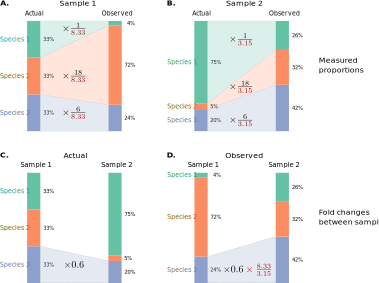
\includegraphics[width=0.9\linewidth]{/tmp/bookdown-differential-abundance-theory/error-proportions} \caption{\textbf{Taxonomic bias creates sample-dependent multiplicative errors in species proportions, which can lead to inaccurate fold changes between samples.} Top row: Error in proportions measured by MGS in two microbiome samples that contain different relative abundances of three species. Bottom row: Error in the estimated fold-change in the third species that is derived from these measurements.}\label{fig:error-proportions}
\end{figure}



\hypertarget{absolute-abundances-cell-densities}{%
\subsection{Absolute abundances (cell densities)}\label{absolute-abundances-cell-densities}}

Various experimental and computational methods have or can be used to supplement MGS measurements so as to convert the relative-abundance information in the read counts into estimates of (absolute) cell densities;
however, these methods can largely be partitioned conceptually into those that use the estimated proportions or the estimated ratios provided by MGS.
The error in density estimates due to taxonomic bias therefore follows that of the proportion and ratio estimates described above.

Proportion-based density estimation is based on the idea that if we know the (true) proportion of a species and the (true) total density of all species, we can multiply these numbers obtain the species' density.
This method therefore involves multiplying the proportion of a species estimated from MGS with an estimate of total microbial density obtain through other means (e.g., through direct cell counting or qPCR of a universal marker gene) to estimate
its density,
\begin{align}
  \label{eq:density-prop-est}
  \hat{\text{density}}_{i}(a) 
  = \hat{\text{prop}}_{i}(a) \cdot \hat{\text{total density}}(a).
\end{align}
The error in this proportion-based density estimate is
\begin{align}
  \label{eq:density-prop-error}
  \hat{\text{density}}_{i}(a) 
  = \text{density}_{i}(a) \cdot \frac{\text{efficiency}_{i}}{\text{mean efficiency}(a)} 
  \cdot \substack{\text{fold error in} \\ \hat{\text{total density}}(a)}.
\end{align}
The multiplicative error consists of two factors: the error in the estimated proportion (due to taxonomic bias in the MGS measurement), and any error in the estimated total density.
In the case of perfect knowledge of the total density, the fold error in proportion-based density estimates varies across samples inversely with the mean efficiency.

Ratio-based density estimation follows from the fact that, in the absence of taxonomic bias, the conversion rate from reads to density is just the sequencing effort of the sample and is thus the same for all species (Equation \eqref{eq:measurement-model}).
Knowing the density of at least one \emph{reference} species therefore enables us to convert from reads to density for all species.
One approach to obtaining such reference species is to add one or more extraneous species in known (typically constant) abundance (a ``spike-in'') to each sample prior to sequencing (REFs).
A second approach is to determine a set of naturally occurring species that are thought to have a constant, though typically unknown, abundance across samples; in this case we can only estimate species' densities relative to these ``housekeeping species'' (REFs).
A third (seemingly untried) possibility is to measure the density of one or more naturally occurring species using a method such as targeted CFU counting, fluorescence flow cytometry or ddPCR directly on cells, or ddPCR or qPCR on extracted DNA.
Given the estimate of the density of reference taxon \(r\), we estimate the density of taxon \(i\) by multipling the ratio of \(i\) to \(r\) in the reads by the density of \(r\),
\begin{align}
  \label{eq:density-ratio-est}
  \hat{\text{density}}_{i}(a) = \frac{\text{reads}_{i}(a)}{\text{reads}_{r}(a)} \cdot \hat{\text{density}}_{r}(a)
\end{align}
(Appendix ??? describes how this equation can be extended to multiple reference species.)
For a constant reference species with unknown density, we can set \(\hat{\text{density}}_{r}(a)\) equal to 1 to estimate density in units of the density of the reference species.
The error in this ratio-based density estimate is
\begin{align}
  \label{eq:density-ratio-error}
  \hat{\text{density}}_{i}(a) 
  = \text{density}_{i}(a) \cdot \frac{\text{efficiency}_{i}}{\text{efficiency}_{r}} 
  \cdot \substack{\text{fold error in} \\ \hat{\text{density}}_{r}(a)}.
\end{align}
Again, the multiplicative error consists of two factors: the error in the estimated ratio (due to taxonomic bias in the MGS measurement), and error in the estimated density of the reference taxa.
So long as the fold error in the reference density is constant across samples, so will be the error in the estimated density of the focal species \(i\).

\begin{itemize}
\tightlist
\item
  Note: The current distinction between proportion- and ratio-based density estimation is incomplete, as the example of spike-in normalization shows: Whether the density of species \(i\) is estimated by Equation \eqref{eq:density-ratio-est}, or by first estimating total density from the ratio of non-spike-in to spike-in reads and then using Equation \eqref{eq:density-prop-est}, the results are mathematically identical. Future revisions should clarify this point.
\end{itemize}

\hypertarget{differential-abundance}{%
\section{How taxonomic bias affects differential-abundance analysis}\label{differential-abundance}}

How do the measurement errors described in the previous section impact our ability to estimate the changes in microbial abundances across samples or between different host and environmental conditions?
Though there are many ways to quantitatively define such change, here we restrict our attention to inferring the multiplicative or (equivalently) log fold change in proportions, ratios, and cell densities, as such inference is ubiquitous in microbiome DA analysis and have more direct ecological interpretations (via the processes of exponential growth and death) than other DA measures.
These measures of DA are also affected by taxonomic bias in our model in a manner that is straightforward to understand in terms of the multiplicative errors described in the previous section.

\hypertarget{change-between-a-pair-of-samples}{%
\subsection{Change between a pair of samples}\label{change-between-a-pair-of-samples}}

Before considering the stereotypical many-sample DA analysis, it is instructive to
consider simplest analysis of differential abundance: the estimation of fold changes in abundance between a pair of samples.
This case is relevant for understanding common visualizations for comparing abundances across individual samples, such as the ubiquitous proportion bar plot and abundances-through-time trajectories within a single host or environment, and conceptually bridges the single-sample results of the previous section to the many-sample case.

The composition-dependent effect of bias on fold error in proportions leads to error in fold-change estimates that is proportional to the inverse change in mean efficiency.
From the error in an individual sample \eqref{eq:prop-error}, it follows that the estimated fold change in proportion of taxon \(i\) from sample \(a\) to sample \(b\) is
\begin{align}
  \label{eq:prop-fc-error}
% \tag*{Fold change in proportion}
\underbrace{\frac{\hat{\text{prop}}_{i}(b)}{\hat{\text{prop}}_{i}(a)}} _\text{estimated FC}
  &= \frac
    {\text{prop}_{i}(b) \cdot \cancel{\text{efficiency}_{i}} / {\text{mean efficiency}(b)}}
    {\text{prop}_{i}(a) \cdot \cancel{\text{efficiency}_{i}} / {\text{mean efficiency}(a)}}
\\[0.5ex]
  &=
  \underbrace{\frac{\text{prop}_{i}(b)}{\text{prop}_{i}(a)}}_\text{actual FC}
  \cdot
  \underbrace{\left[\frac{\text{mean efficiency}(b)}{\text{mean efficiency}(a)}\right]^{-1}}_\text{fold error}
  .
\end{align}
The sample-independent efficiency factor of the error cancels, but the sample-dependent mean efficiency does not, leaving an error equal to the inverse of the change in the mean efficiency from \(s\) to \(t\).

The bottom row of Figure \ref{fig:error-proportions} illustrates how variation in mean efficiency leads to error in the inferred fold changes between a pair of samples.
The mean efficiency decreases by a factor of 2.6 (FC: 0.4X) from Sample 1 to Sample 2.
Consequently, the FC of each species is measured to be 2.6X larger than the true value.
Though the fold error for all species is the same, the implications depend on the actual FC and correspond to three distinct types of error: an increase in magnitude, a decrease in magnitude, and a change in direction (or sign).
We can see each type of error in Figure 2.
For Species 1, which increases and thus moves in the opposite direction of the mean efficiency, we see an increase in magnitude of the estimated FC (actual FC: 2.3X, measured FC: 6.5X).
For Species 2, which decreases and thus moves in the same direction as the mean efficiency but by a larger factor, we see an decrease in magnitude (actual FC: 0.15X, measured FC: 0.44X).
For Species 2, which decreases by a smaller factor than the mean efficiency, we see a change in direction (actual FC: 0.6X, measured FC: 1.8X), such that the species actually appears to increase!

In contrast, because species ratios are distorted by a constant factor, their measured fold changes remain accurate.
The fold error in Equation \eqref{eq:ratio-error} completely cancels when we divide the ratio measured for one sample \(a\) by another sample \(b\).

If other error sources remain negligible, than this dichotomy continues to apply to proportion- and ratio-based density estimates.
The inferred FCs in proportion-based density estimates will be incorrect by a factor equal to the inverse fold change in the mean efficiency, creating magnitude and/or directional errors.
Moreover, any species with a constant density will appear to vary inversely with the mean efficiency.
In contrast, fold changes in ratio-based density estimates remain accurate.

\hypertarget{regression-analysis-of-many-samples}{%
\subsection{Regression analysis of many samples}\label{regression-analysis-of-many-samples}}

DA analysis of many samples across host or environmental conditions can typically be framed as a regression problem, in which we analyze the relationship between a microbial \emph{response variable}, such as log density of some focal species \(i\), and one or more \emph{covariates}, such the pH or temperature of the sampled environment or whether the sample is from a healthy or sick person.
A substantial fraction of DA analyses use minor elaborations on the simple linear regression model, which for a response of log species density can be written
\begin{align}
  \label{eq:regression}
  \log \text{density}_i(a) = \alpha + \beta x(a) + \varepsilon_i(a).
\end{align}
Here \(x\) is a continuous covariate (e.g.~pH) or a binary covariate (e.g.~\(x=1\) for treated patients and \(x=0\) for controls), \(\alpha\) and \(\beta\) are regression coefficients, and \(\varepsilon_i(a)\) is a mean-zero random variable that reflects the residual (unexplained) variation in the response (log density of species \(i\)).
Our interest is usually in the coefficient \(\beta\) (slope or average difference between conditions) that describes how the species' abundance changes with \(x\), while the intercept \(\alpha\) captures differences in the baseline abundance and---we hope---measurement efficiency among species.
How does taxonomic bias under our measurement model affect estimates of \(\beta\) in the simple linear regression?

Consider the case where the response is log density that has been estimated using proportion-based density estimation (Equation \eqref{eq:density-prop-est}) with error-free estimates of the total density.
If the true log density follows the regression Equation \eqref{eq:regression}, then it follows from Equation \eqref{eq:density-prop-error} the estimated log density equals
\begin{align}
  \label{eq:regression-error}
  \log \hat{\text{density}}_i(a)
%  &= \alpha + \beta x(a) + \varepsilon_i(a) + \log \text{efficiency}_i - \log \text{mean efficiency}(a)
  = [\alpha + \log \text{efficiency}_i] + [\beta - \log \text{mean efficiency}(a)] x(a) + \varepsilon_i(a).
\end{align}
This equation shows that the species-specific portion of the error affects the intercept term while the sample-specific portion (log mean efficiency) affects the slope term.
Thus, as in the case of fold changes between two samples (Equation \eqref{eq:prop-fc-error}), it is the variation in the (log) mean efficiency across samples that we must worry about distorting our DA results.

The variation in measurement error created by the log mean efficiency impacts the point estimate and precision of the regression coefficient \(\beta\).
Box \ref{regression-error} mathematically describes this effect for estimation method of Ordinary Least Squares (OLS) and Maximum Likelihood Estimation (MLE) and Figure \ref{fig:regression-example} illustrates using simulated data.
Variation in the log mean efficiency that is associated with the covariate \(x\) creates a systematic error in the estimated slope \(\hat \beta\) equal to the negative of the (scaled) covariance of log mean efficiency with \(x\).
The absolute error is the same for all species; however, its relative value depends on the magnitude of the covariance of the log mean efficiency with \(x\) relative to that of the response (here, \(\log \text{density}_{i}\)) with \(x\) or, equivalently, the relative magnitudes of their slopes.
As in the case of fold changes between pairs of samples, the net effect can be decreases in magnitude (Species 9, 10, and 1 in Figure \ref{fig:regression-example}), changes in sign (Species 5), or increases in magnitude (remaining species) depending on these relative values.
Variation in the log mean efficiency that is uncorrelated with \(x\) does not systematically distort \(\hat \beta\) but does affect its precision, typically leading to increased standard errors as the variation in log mean efficiency effectively acts as an additional source of noise in measured abundance (Figure \ref{fig:regression-example} D).
The exception is for species whose residual variation is strongly positively correlated with that of log mean efficiency (here, Species 9), which can appear to have less random variation and receive standard errors that are too small.
Decreased magnitudes and increased standard errors can both cause associations to be missed that would otherwise have been detected (Species 10 and 1), while increased magnitudes can turn weak or statistically insignificant associations into strong and statistically significant ones (Species 7, 6 and 4).

With this understanding in place, we briefly summarize how taxonomic bias affects estimation of the simple linear model in other abundance types.
The results for proportion-based density estimates with accurate total densities also apply to LFC analysis of proportions.
Similar results apply to microbiome regression tools (such as corncob; \protect\hyperlink{ref-martin2020mode}{Martin, Witten, and Willis} (\protect\hyperlink{ref-martin2020mode}{2020})) that perform regression on the logit (instead of log) proportion of a species; however,
the mean efficiency of the entire sample must instead be replaced with the mean efficiency among all species excluding the focal species, which causes the absolute error in regression coefficients to vary somewhat across species.
Because ratios and ratio-based densities are subject to consistent multiplicative error, in analysis of log ratios and the log densities derived from them, only the estimated intercept \(\hat \alpha\) is affected by taxonomic bias, while the point estimate and standard error of the estimated slope \(\hat \beta\) remain unaffected.

\begin{figure}
\centering
\includegraphics{/tmp/bookdown-differential-abundance-theory/regression-example.pdf}
\caption{\label{fig:regression-example}\textbf{Taxonomic bias distorts multi-sample differential abundance inference when the mean efficiency of samples is associated with the covariate of interest.} This figure shows the results of a regression analysis of simulated microbiomes consisting of 50 samples and 10 species from two environmental conditions indexed by \(x=0\) and \(x=1\). In this simulation, the species with the largest efficiency (Species 9) also has the largest positive LFC, which drives the positive association of the log mean efficiency with the condition (shown in Panels A and B). This positive LFC in the log mean efficiency induces a systematic negative shift in the estimated LFCs of all species (Panels C and D). Panel D shows the mean LFC (points) with 95\% confidence intervals (CIs), for each species estimated from either the actual or the measured densities. The error (difference in LFC estimates on measured and actual) equals the negative LFC of the mean efficiency (shown in Panel B).}
\end{figure}



\hypertarget{regression-error}{%
\subsection{Box: Error in estimated regression coefficients and standard errors}\label{regression-error}}

Results from statistics on regression under measurement error can help us understand the effect of bias on DA regression analysis.

Consider Equation \eqref{eq:regression} for the simple linear regression of log density of a species \(i\) on covariate \(x\).
Let \(y\) stand for the actual log density of a focal species \(i\), \(z\) stand for the log density that we've measured, and \(d = z - y\) equal the difference between the two, which here is the log efficiency of species \(i\) minus the log mean efficiency of the sample.
Let \(s_{xy}\) denote the sample covariance between variables \(x\) and \(y\), \(s^{2}_{x} = s_{xx}\) and \(s_{x}\) denote the sample variance and standard deviation, and \(r_{xy} = s_{xy}/(s_{x}s_{y})\) denote the sample correlation.

The ordinary least squares (OLS) and maximum likelihood (MLE) estimates of the slope of \(z\) equals the sample covariance of \(z\) and \(x\) divided by the sample variance in \(x\) or, equivalently, the sample correlation of \(z\) and \(x\) multiplied by the ratio of their sample standard deviations,
\begin{align}
  \hat \beta_z = \frac{s_{zx}}{s^2_x} = r_{zx} \cdot \frac{s_y}{s_x}.
\end{align}
From the (bi)linearity of sample covariances it follows that
\begin{align}
  \hat \beta_z 
  = \frac{s_{yx}}{s^2_x} + \frac{s_{dx}}{s^2_x} 
  = \frac{r_{yx} s_y}{s_x} + \frac{r_{dx} s_d}{s_x} 
  = \hat \beta_y + \hat \beta_d,
\end{align}
where \(\hat \beta_y\) and \(\hat \beta_d\) denote the slope estimates for \(y\) and \(d\) (were these values to be known).
The absolute error in the estimate \(\hat \beta_{z}\) of \(\hat \beta_{y}\) is therefore \(\hat \beta_{d}\); it is large in a practical sense when \(\hat \beta_{d}\) is large (in absolute value) compared to \(\hat \beta_{y}\), which corresponds to the covariance of \(d\) with \(x\) being large compared to the covariance of \(y\) with \(x\).

In our case, the covariance of \(d\) equals the negative of the covariance of log mean efficiency with \(x\).
The absolute error (i.e., the \emph{bias} in a statistical sense) in \(\hat \beta\) is equals the negative covariance of log mean efficiency scaled by the variance in \(x\).
This absolute error is the same for all species; however, its practical significance varies depending on its magnitude relative to that of the slope of the actual log densities.
For species that covary with \(x\) more strongly than the log mean efficiency, the error will be relatively small.
This situation might occur either because the mean efficiency varies relatively little across samples or because its variation is relatively less correlated with \(x\) compared to the log density of the focal species.

We can similarly understand the impact of measurement error on the precision of our slope estimates.
The OLS and MLE estimated standard error in \(\hat \beta\) are both approximately
\begin{align}
  \hat{\text{se}}(\hat \beta)
  \approx \frac{s_{\hat \varepsilon}}{s_x \sqrt{n}},
\end{align}
where \(s_{\hat \varepsilon}\) is the sample standard deviation of the residuals
(\protect\hyperlink{ref-wasserman2004allo}{Wasserman} (\protect\hyperlink{ref-wasserman2004allo}{2004}) Chapter 13).
The sample residuals of \(z\), \(y\), and \(d\) have a similar relationship to the regression coefficient estimates,
\begin{align}
  \hat \varepsilon_z 
    &\equiv z - \hat \beta_z x
  \\&= (y + d) - (\hat \beta_y + \hat \beta_d) x
  \\&= (y - \hat \beta_y x) + (d - \hat \beta_d x)
  \\&= \hat \varepsilon_y + \hat \varepsilon_d.
\end{align}
(Note, here I've omitted the subscript indicating the dependence on the sample.)
It follows that the sample variances of the residuals of \(z\), \(y\), and \(d\) are related through
\begin{align}
  s^2_{\hat \varepsilon_{z}} 
  = s^2_{\hat \varepsilon_{y} + \hat \varepsilon_{d}}
  = s^2_{\hat \varepsilon_{y}} + s^2_{\hat \varepsilon_{d}} + 2 s_{\hat \varepsilon_{y} \hat \varepsilon_{d}}.
\end{align}
The standard deviation of the \(z\) residuals is increased above that of the \(y\) residuals when the \(d\) residuals are either uncorrelated or positively correlated with the \(y\) residuals, but may be decreased when the \(y\) and \(d\) residuals are negatively correlated.

In our case, the \(d\) residuals equal the negative residuals of the log mean efficiency.
It is plausible that for most species, their residual variation will have a small covariance with log mean efficiency and the net effect of variation in the mean efficiency will be to increase the estimated standard errors, as occurs with most species in Figure \ref{fig:regression-example}.
However, high-efficiency species that vary substantially in proportion across samples may be strongly positively correlated with log mean efficiency such that the estimated standard errors decrease, as we see with Species 9 in Figure \ref{fig:regression-example}.

\hypertarget{implications}{%
\section{Implications for real-world inference~}\label{implications}}

Partial but not full canceling of the effect of bias in proportion-based analyses, such that possible to have spurious results in principle; but what about in practice?
Predicting how frequently or which results are likely to be majorly affected is difficult because it depends on the joint variation in efficiencies of species and species abundance dynamics, both of which are poorly understood in most to all biological systems.
However, through a combination of theoretical considerations, hypothetical scenarios, and real case studies we can begin to develop an understanding or the relevant considerations and build framework for improving our understanding as our knowledge of these dynamics improves.

\hypertarget{systematic-error-in-slope-or-lfc-estimates}{%
\subsection{Systematic error in slope or LFC estimates}\label{systematic-error-in-slope-or-lfc-estimates}}

Recall from Section \ref{differential-abundance} that the error in the slope or LFC in a DA regression analysis is proportional to the covariance of the log mean efficiency with the covariate.
This covariance can be split into two components: the standard deviation of (log) mean efficiency and its correlation with the covariate.
Hence when considering whether taxonomic bias creates large error, it can be useful to separately ask whether the mean efficiency is likely to vary across samples and whether it is likely to be correlated with a covariate of interest.

One approach to studying the mean efficiency empirically is to analyze data from studies for which control measurements allow direct measurement of species' efficiencies.
\protect\hyperlink{ref-brooks2015thet}{Brooks et al.} (\protect\hyperlink{ref-brooks2015thet}{2015}) performed 16S rRNA gene sequencing of mock communities of seven bacterial species thought to play a critical role in the human vaginal microbiome with the MGS protocol developed for the Vaginal Human Microbiome Project (VaHMP). \protect\hyperlink{ref-mclaren2019cons}{McLaren, Willis, and Callahan} (\protect\hyperlink{ref-mclaren2019cons}{2019}) later used this data to estimate the efficiencies of these seven species and develop a method to use these estimates to infer the true compositions of natural samples (see Section @ref(\#calibrate-compositions)).
SI Analysis (MOMS-PI) uses these estimated efficiencies to correct the compositions and explore the implied variation in mean efficiency in the VaHMP's Multi-Omic Microbiome Study: Pregnancy Initiative (MOMS-PI) \protect\hyperlink{ref-fettweis2019thev}{Fettweis et al.} (\protect\hyperlink{ref-fettweis2019thev}{2019}).
The vaginal microbiome during pregnancy is characterized by relatively low diversity, often with a single \emph{Lactobacillus} species often forming a majority of reads (considered to be the healthy state) but with occasional shifts to high proportions of other species, such as \emph{Gardnerella vaginalis}, \emph{Atopobium vaginae}, and \emph{Streptococcus agalactiae}, which are thought to cause or indicate poor vaginal health and increased risk of preterm birth.
The analysis of \protect\hyperlink{ref-mclaren2019cons}{McLaren, Willis, and Callahan} (\protect\hyperlink{ref-mclaren2019cons}{2019}) showed that the efficiencies of two common \emph{Lactobacillus} species, \emph{L. crispatus} and \emph{L. iners}, were 20-30X greater than that of \emph{G. vaginalis}, \emph{A. vaginae}, and \emph{S. agalactiae}.
Analysis of microbiome trajectories of a single patient across visits indicates that the mean efficiency typically decreases by a factor of 3-10X when the community shifts from a high to low-\emph{Lactobacillus} state.
(NOTE: This is a super preliminary claim based on looking at just one woman, and is just a placeholder)
Decreases in mean efficiency during transitions from \emph{Lactobacillus} to \emph{Gardnerella} dominance can be expected to be even more extreme for commonly-used vaginal microbiome primers that fail to amplify \emph{Gardnerella}.

A second study in which control communities make it possible to directly analyze the impact of taxonomic bias in experimental samples was performed by \protect\hyperlink{ref-leopold2020host}{Leopold and Busby} (\protect\hyperlink{ref-leopold2020host}{2020}).
To study the interactions between a host plant and its fungal commensals and pathogen, the authors inoculated trees with a fungal synthetic community and later exposed plants to a fungal pathogen.
The authors used ITS amplicon sequencing to measure communities before and after infection, along with mock communities which they used to estimate the species efficiencies with the method of \protect\hyperlink{ref-mclaren2019cons}{McLaren, Willis, and Callahan} (\protect\hyperlink{ref-mclaren2019cons}{2019}).
(DNA mocks were used, so that bias due to DNA extraction is not included, but other major bias sources such as PCR and ribosomal copy-number-variation are included.) The pathogen was 10X more efficiently measured than the median commensal and 40X more efficiently measured than the lowest-efficiency commensal.
A re-analysis of their data (SI Analysis) shows that the mean efficiency varies by ??? in pre-infection communities and by an average of ??? pre- and post-infection, with the latter driven by the dramatic increase in the high-efficiency pathogen.

These case studies indicate that one mechanism for variability in the mean efficiency is swings between very high (\(\sim 1\)) and low (\(\ll 1\)) proportions of species with particularly high or low efficiencies.
In highly diverse ecosystems, as seen in soil and the human gut (CHECK), one species rarely dominates within a given sample and so such large swings are not possible.
We might therefore think that the mean efficiency will remain fairly stable in these settings.
In fact, one can show mathematically that in randomly assembled communities, the mean efficiency becomes more stable as (Inverse Simpson) diversity increases, as the mean effectively averages over a greater number of species.
Real communities do not assemble randomly, however.
Variance in the mean efficiency may remain high if environmental filtering leads to different groups of organisms dominating in different environments, particularly if shared phenotypic values or evolutionary history causes these groups to differ in their efficiencies as well as their ecology.
For example, gut microbiomes typically have high diversity at the species level but are dominated by just a small number of phyla, and two in particular: The Bacteroidetes and the Firmicutes, the ratio of which varies substantially across individuals (CHECK).
Many DNA extraction protocols have been found to more efficiently lyse Gram-negative Bacteroidetes species than Gram-positive Firmicutes species (though variation can also be substantial within phyla, \protect\hyperlink{ref-mclaren2019cons}{McLaren, Willis, and Callahan} (\protect\hyperlink{ref-mclaren2019cons}{2019})).
Gut samples with large differences in their Bacteroidetes and Firmicutes proportions may therefore have large variation in mean efficiency even if the individual species within each phylum never reach a large proportion.
On the other hand, competitive-exclusion dynamics can favor more stable taxonomic and/or phenotypic compositions across samples and might thereby drive a more stable mean efficiency than under random assembly

Systematic error in DA results requires that the variation in log mean efficiency is correlated with the covariate.
The examples above each suggest plausible biologically-significant scenarios in which such correlations might arise.
For example, in the vaginal microbiome a decline in \emph{Lactobacillus} and rise of species including \emph{Gardnerella vaginalis} is associated with preterm birth in pregnant women; hence the variation in mean efficiency driven by these species may also create an association of mean efficiency with preterm status.
In the plant-fungal experiment of \protect\hyperlink{ref-leopold2020host}{Leopold and Busby} (\protect\hyperlink{ref-leopold2020host}{2020}), the increase in pathogen proportion after infection leads to a large increase in the mean efficiency over time, which systematic increases the observed decline in the proportions of commensal species (SI Analysis).
The ratio of Bacteroidetes to Firmicutes has been linked to several host traits and health conditions, and thus the variation in efficiency between these two phyla may also drive an association of mean efficiency with these traits.

Are there general mechanisms by which we might expect associations to arise between mean efficiency and the covariates commonly of interest in microbiome studies?
One possibility is that the ecology and measurement efficiency of species may become correlated simply due to shared evolutionary history.
A species' efficiency is heavily influenced by genetically determined traits such as cell-wall structure, ribosomal-operon copy number, sequence in a primer-targeted region, GC content, and even whether the species is present in a given taxonomic database.
Shared evolutionary history among phylogenetically-close species is expected and has been observed to create positive associations in these traits among more closely related species, such that we should expect a significant degree of phylogenetic conservation in efficiency.
Meanwhile, the same shared evolutionary history creates phylogenetic conservation in ecological traits that drives species abundance dynamics.
In this way, we may expect evolution to lead to a situation in which groups of species with similar efficiencies have similar shifts in abundance between conditions, creating the potential for commensurate shifts in mean efficiency.
For example, a change in diet that favors Bacteroidetes species relative to Firmicutes based on the resulting gut conditions will also increase the relative abundance of easy-to-lyse species.

Associations between efficiency and abundance can also arise more directly when a single microbial trait affects both.
For example, microbes at the ocean floor are slowly buried, sinking into a low nutrient, low oxygen environment.
\protect\hyperlink{ref-lloyd2020evid}{Lloyd et al.} (\protect\hyperlink{ref-lloyd2020evid}{2020}) estimate the log fold change in the estimated absolute abundance of various taxa with sediment depth (as a proxy for time) to determine which taxa are able to persist and even grow in this difficult environment.
It is plausible that microbes with tougher cell walls would tend to persist longer (alive or dead) in the sediment, while at the same time being more difficult to extract DNA from than microbes with weaker cell walls.
As the relative abundance of tougher species increases with depth, the mean extraction efficiency decreases.
This decrease would increase the inferred log fold changes and could lead to inferred growth of taxa that are actually just persisting or even slowly dying off.
Another example of a trait that might simultaneously affect efficiency and relative abundance is ribosomal copy number, which increases the measurement efficiency in ribosomal amplicon experiments and is also linked to differences in ecology and population dynamics among species.

The biological significance of the error in \(\hat \beta\) depends on the relative magnitude of the LFC (or covariance with the covariate \(x\)) in the focal species vs in the mean efficiency.
It may generally be true that the largest species LFCs in a DA analysis, which are often of primary interest in a microbiome study, will tend to be larger than the LFC of the mean efficiency, at least in high-diversity settings.
(This seems intuitively likely and true in examples, but I haven't analyzed it much mathematically and don't have a firm handle on this question.)
Further investigation into this question may improve our confidence in the top hits identified in published DA analyses meeting certain conditions.
However, we must remain weary of cases (as in the vaginal-microbiome and plant-fungal-interactions examples above) in which a shift in a single species can drive large changes in mean efficiency and lead to significant errors for all other species.
The experimental and computational methods discussed in Section \ref{solutions} can mitigate taxonomic bias in these clearly-problematic cases while also helping to amass empirical evidence on the conditions in which bias is unlikely to cause major inferential errors.

\begin{itemize}
\tightlist
\item
  Todo: Address DA analysis of aggregate (or synthetic) taxa, such as phyla, which may be prone to errors due to changes in the species-level make-up of the taxon.
\end{itemize}

\textbf{Error in total-density measurements:}

So far we have ignored error in total-density measurements that are used to convert estimated proportions to estimated densities;
however, in reality these measurements are likely to contain substantial systematic error that can either worsen or improve the error in LFC estimates.

\begin{itemize}
\tightlist
\item
  Todo: Add to previous section or Appendix with the relevant theory.
\end{itemize}

To understand how, we can consider the question of whether bulk 16S qPCR or flow cytometry is a more appropriate method of measuring total bacterial density for use in proportion-based density measurement (\protect\hyperlink{ref-galazzo2020howt}{Galazzo et al.} (\protect\hyperlink{ref-galazzo2020howt}{2020}), \protect\hyperlink{ref-jian2021comm}{Jian, Salonen, and Korpela} (\protect\hyperlink{ref-jian2021comm}{2021})).
16S rRNA-gene qPCR measures the concentration of 16S rRNA gene copies in the extracted DNA and is therefore affected by variation among species in DNA extraction efficiency, 16S copy number, and primer-binding and amplification efficiency.
For example, \protect\hyperlink{ref-mclaren2019cons}{McLaren, Willis, and Callahan} (\protect\hyperlink{ref-mclaren2019cons}{2019}) found that the product of extraction efficiency and 16S copy number for \emph{Lactobacillus iners} was 20X larger than \emph{Gardnerella vaginalis} (CHECK NUMBERS), such that we should expect samples dominated by \emph{L. iners} to result in qPCR estimates 10-20X higher than equally dense samples dominated by \emph{G. vaginalis}.
These observations suggest that 16S qPCR is a poor proxy for fold changes in total bacterial density.
Yet, as recently suggested by \protect\hyperlink{ref-jian2021comm}{Jian, Salonen, and Korpela} (\protect\hyperlink{ref-jian2021comm}{2021}), this taxonomic bias in qPCR may simultaneously make it a good measure of total density for use with 16S amplicon sequencing for proportion-based density estimation.
16S amplicon sequencing shares these same sources of bias and so is likely to have species efficiencies highly similar to those for the qPCR measurements, which we can predict to cause the mean 16S-qPCR efficiency to closely follow the mean 16S-sequencing efficiency, such that the error induced by one largely cancels the error induced by the other (Ref Appendix).
In contrast, species-specific efficiencies in bulk cell counting are less likely to be strongly correlated with those from 16S sequencing.
Even supposing cell counting were to provide perfectly accurate measures of total density, it may actually perform worse than qPCR for DA analysis of proportion-based density estimation precisely because the error does not mirror that in the 16S measurement.

On the other hand, bulk or targeted measurement (or DNA spike-ins) that occurs post DNA-extraction is subject to other error that is not likely to counter that of the 16S-based proportion estimates.
The yield of DNA extraction can show highly random variation and also be highly non-linear (as a function of cellular biomass) at high concentrations.
This features create error that is unlikely to offset the variation in mean efficiency in the 16S sequencing (todo: clarify why).
Targeted measurement of cells and cellular spike-ins, discussed in Section \ref{solutions}, can avoid this issue while also facilitating ratio-based analysis while (unlike bulk cell counting) remaining robust mean-efficiency variation.

\hypertarget{loss-of-power-and-precision-stub}{%
\subsection{Loss of power and precision (stub)}\label{loss-of-power-and-precision-stub}}

Variation in mean efficiency that is not associated with covariates can still majorly hinder the goals of microbiome studies by causing reductions in the precision of LFC estimates and the power to detect true associations of a given size.

\begin{itemize}
\tightlist
\item
  Illustrate with case studies?
\item
  Mention counting noise as an important factor that we've so far ignored but that can interact with taxonomic bias to lead to very low precision in LFC estimates. Low efficiency can put a species below the detection limit set by sample read depth, making it impossible to get precise LFCs. Study-specific efficiencies can explain why associations often do not replicate across studies. Example: \emph{Gardnerella vaginalis} associations are not detected in certain vaginal microbiome studies that used V13 primers which we now know are bad at amplifying it.
\item
  Conclude with a nod to the value of the solutions in Section \ref{solutions} to address these issues: Correcting the errors caused by mean-efficiency variation can improve precision, and bias-sensitivity analysis and bias-aware meta-analysis can give a better sense of the increased uncertainty in LFC estimates due to unknown efficiencies, thereby helping us to understand the increased rate of false positives and/or the larger range of LFC estimates that are compatible with the observed data than what is implied by a bias-free model.
\end{itemize}

\hypertarget{solutions}{%
\section{Potential solutions}\label{solutions}}

The theoretical results from Section \ref{differential-abundance} suggest a number of potential methods to avoid, correct, or otherwise mitigate the errors created by taxonomic bias.
We present five that seem particularly promising:
The first three are method for correcting or otherwise account for the effects of taxonomic bias to obtain more accurate DA results, whereas the second two treat the measurement efficiencies as unknown parameters and seek to understand the additional uncertainty they create, either in the results of individual studies or in joint analysis of multiple studies that used different MGS protocols.

\hypertarget{calibrate-compositions}{%
\subsection{Calibrate compositions using community controls}\label{calibrate-compositions}}

The most complete but experimentally challenging approach to mitigating taxonomic bias involves directly measuring the efficiencies of individual species using control samples (\protect\hyperlink{ref-mclaren2019cons}{McLaren, Willis, and Callahan} (\protect\hyperlink{ref-mclaren2019cons}{2019})).
Suitable controls are any community sample whose composition (species identity and relative abundances) has been previously characterized, either by construction (in the case of constructed `mock' communities) or by measurement with a \emph{reference protocol} chosen to serve as a measurement standard.
These controls, when measured alongside the target experimental samples, can be used to estimate the relative efficiencies among the superset of species across the control samples.
The estimated efficiencies can then be used to calibrate the measured relative abundances among the control species in the target samples to the chosen measurement standard, by simply dividing the species' read counts by their corresponding efficiencies or using a more sophisticated statistical modeling framework.
These calibrated compositions can then be used for arbitrary downstream microbiome analyses, including DA analysis.
Calibration of species not in the controls requires first imputing their efficiencies from the control measurements, for example using phylogenetic relationships, genetic characteristics (such as 16S copy number), and/or phenotypic properties (such as cell-wall structure).
Though such imputation is conceptually straightforward to implement, its reliability and utility remain untested.

\begin{itemize}
\tightlist
\item
  The above states the approach; can add description/discussion of application to the MOMS-PI and \protect\hyperlink{ref-leopold2020host}{Leopold and Busby} (\protect\hyperlink{ref-leopold2020host}{2020}) cases and developments and challenges in availability of control communities
\end{itemize}

\hypertarget{use-ratio-based-abundance-measurement}{%
\subsection{Use ratio-based abundance measurement}\label{use-ratio-based-abundance-measurement}}

The DA analyses we consider don't need accurate estimates of relative abundances within individual samples---they only require accurate fold changes across samples.
Section \ref{differential-abundance} showed that fold changes in species ratios and ratio-based density estimates can remain accurate even when taxonomic bias distorts the values in individual samples.
Hence a solution is to use to analyze variation in ratios and ratio-based density estimates.
For the latter, practical options include

\begin{itemize}
\tightlist
\item
  spike-ins of extraneous species at constant and/or known density
\item
  housekeeping taxa, stipulated or computationally identified as having a constant density across samples
\item
  targeted measurement of specific taxa
\end{itemize}

TBD what further discussion or illustration to have here.

\hypertarget{calibrate-fold-changes-using-measurements-of-targeted-taxa}{%
\subsection{Calibrate fold changes using measurements of targeted taxa}\label{calibrate-fold-changes-using-measurements-of-targeted-taxa}}

In some cases, we may still which to use a proportion-based approach to analyzing variation in density.
For example, in some systems measuring total cell concentration may be easier than implementing a spike-in experiment or determining a set of reference species to directly measure for which at least one species is present in all samples.
In this case, targeted measurements of one or more reference species can be used to validate and/or correct the fold changes or regression coefficients infered from the proportion-based densities.
Recall that the error in proportion-based log fold changes (LFCs) is shared among species and is equal to the inverse LFC fold change in mean efficiency (Equations \eqref{eq:prop-fc-error} and \eqref{eq:regression-error}; Figure \ref{fig:regression-example}D).
Consequently, an accurate LFC of one or more reference species can serve as a general validation or used to correct the LFCs of all species.

\begin{itemize}
\tightlist
\item
  Note: I may not correctly understand the next example, since I don't yet see how this interpretation of Table 1 meshes with Figure 4
\end{itemize}

We illustrate this idea with an example from the study by \protect\hyperlink{ref-lloyd2020evid}{Lloyd et al.} (\protect\hyperlink{ref-lloyd2020evid}{2020}) described in Section \ref{implications}, which estimated doubling times for various taxa from the measured log increase in cell density with burial time in marine sediments.
The primary analysis, which used proportion-based density estimates, was supported by targeted measurements (qPCR) of 16S concentration for several bacterial and archeal taxa (CHECK).
In Core 30, the doubling time estimated for the Archaeal phylum Bathyarchaeota was estimated to be 10.1 years (CHECK) using the proportion-based densities and 10.3 years by qPCR (\protect\hyperlink{ref-lloyd2020evid}{Lloyd et al.} (\protect\hyperlink{ref-lloyd2020evid}{2020}) Table 1 and Figure 4).
These doubling times correspond to highly similar estimated slopes of log density per year of \(1/10.1 \approx 0.99\) and \(1/10.3\approx 0.97\).
The difference between these slopes, \(\approx 0.02\), estimates the slope of the mean efficiency.
It's small value suggests little systematic variation in mean efficiency with burial time and hence little systematic bias in the estimated doubling times derived from the proportion-based density estimates.
In this case, close agreement in the DA results across methods for a specific taxon suggests that variation in sample mean efficiency did not significantly distort the MGS-based results and hence provides a degree of validation for all taxa, not just the taxa with targeted measurements.
(An important caveat for this example is that this analysis assumes consistent efficiencies at the higher taxonomic levels used for qPCR measurement and MGS analysis performed by \protect\hyperlink{ref-lloyd2020evid}{Lloyd et al.} (\protect\hyperlink{ref-lloyd2020evid}{2020}).)
Here we compared summary statistics; however, in principle a joint statistical analysis of targeted and proportion-based density measurements would provide more statistical power to estimate and correct the effects of variation in the mean efficiency across samples and provide calibrated fold change and regression estimates for all taxa {[}APPENDIX{]}.

\hypertarget{perform-a-bias-sensitivity-analysis}{%
\subsection{Perform a bias sensitivity analysis}\label{perform-a-bias-sensitivity-analysis}}

What can we do for experiments that have been conducted without control communities, targeted control measurements, or spike-ins?
One approach is to conduct a bias sensitivity analysis to probe the extent and way in which the results of a DA analysis are sensitive to different possible taxonomic biases in our experiment.

A straightforward approach to bias sensitivity analysis is to use computer simulation to randomly generate efficiency vectors, each of which is used to calibrate the MGS measurements.
These calibrated MGS measurements represent the true compositions under the hypothesized taxonomic bias.
By re-running our DA analysis and comparing results across these simulated datasets, we can begin to understand how our initial results might be influenced by the strength and structure of the taxonomic bias in our experiment.

The simulated efficiency vectors may be generated to reflect certain hypotheses about bias in the given system.
The utility of such simulations can increase the more we learn about the magnitude of bias in different systems and the taxonomic and protocol features that determine it.
Future work in developing tools and methods for simulating efficiency vectors and performing bias sensitivity analyses could be a valuable way to assay and improve the reliability of microbiome results---for differential abundance and microbiome analyses more generally.

\hypertarget{use-bias-aware-meta-analysis}{%
\subsection{Use bias-aware meta-analysis}\label{use-bias-aware-meta-analysis}}

So far we have considered analysis of samples subject to the same taxonomic bias;
however, meta-analysis of microbiome samples measured across multiple studies must often contend with a diversity of protocols and hence taxonomic biases in different groups of samples.
This inconsistency in taxonomic bias across studies poses a problem even for ratio-based analyses where the effects of bias might cancel within a study.

A potential solution is to perform a bias-aware meta-analyses that jointly analyzes multiple data from studies while explicitely acknowledges the distinct, unknown taxonomic bias in each study.
Parametric microbiome meta-analysis models already include sets of species-specific latent parameters to model ``batch effects''---amorphous differences in the measurements of each study.
By configuring these models so that these latent parameters correspond to the study and species specific efficiencies, we can increase the biological interpretability of these models and gain ability to determine whether disageements in DA results across studies are due to differences in taxonomic bias or other differences (such as host cohort or study design).
Using a biophysically motivated model parameterization may also lead to performance gains in terms of increased explanatory power for a given model complexity, as seen for models of mock community measurements by \protect\hyperlink{ref-mclaren2019cons}{McLaren, Willis, and Callahan} (\protect\hyperlink{ref-mclaren2019cons}{2019}), which can increase improve our ability to find reproducible microbial associations in a given meta-study.

\hypertarget{appendix-appendix}{%
\appendix \addcontentsline{toc}{section}{\appendixname}}


\hypertarget{models}{%
\section{Measurement models}\label{models}}

Deterministic measurement error models that extends the \protect\hyperlink{ref-mclaren2019cons}{McLaren, Willis, and Callahan} (\protect\hyperlink{ref-mclaren2019cons}{2019}) model of metagenomics measurement to 1) describe absolute as well as relative abundance, 2) include spike-in taxa, and 3) include supplementary measurements of bulk and targeted (absolute) abundance.

\hypertarget{actual-abundances-and-general-notation}{%
\subsection{Actual abundances and general notation}\label{actual-abundances-and-general-notation}}

(For now) Number of samples = J; Number of taxa = I.

\(A_{ij}\) is the actual absolute abundance of taxon \(i\) in sample \(j\), in the target units.
For variables that hold matrixes or vectors, capital letters denote absolute abundances and lower case letters denote proportions.
Thus \(a_{ij}\) is the matrix of actual relative abundances in terms of cells as a proportion of the total amount of cells in the sample; \(a_{ij} = A_{ij} / A_{Tj}\).
Let \(A_{Tj}\) (or \(A_{\cdot j}\)??) be the total abundance in sample \(j\), \(A_{Tj} = \sum_i A_{ij}\).
For a subset of taxa \(Q \subset \{1, \dots, I\}\), define \(A_{Qj} \equiv \sum_{i \in Q} A_{ij}\) to be the total abundance of the taxa in \(Q\).

Unless specified otherwise, \(A\) always refers to abundance in the original sample material, not in extracted DNA.
I will assume the target units are concentration of cells per unit mass. However, other units (such as biomass per volume) may be relevant.

To consider various addition information that can be used for absolute abundance inference, I let \(B\) denote bulk abundance measurements (such as via flow cytometry or broad-range 16S qPCR), \(S\) denote the known taxon abundances of a spike-in, and \(T\) denote the abundances of a set of taxa made via targeted measurement.
I let \(R \subset \{1, \dots, I\}\) denote the set of \emph{reference taxa} whose abundance is known independently from the metagenomics measurement (up to experimental bias factors) because they were spiked at a known density, subjected to a targeted measurement, or have been determined through some other means to have a constant or known abundance across samples.

Bias vectors \(B^{(P)}\) are vectors of length \(I\) indicating the taxon-specific bias associated with a measurement protocol \(P\).
I generally assume these to be sample-independent.
An overbar denotes the average value over taxa weighted by actual abundance; i.e., \(\bar B_j = I^{-1} \sum_i B_i a_{ij}\).
An overbar and a subcript set of taxa indicates the mean bias within that subset: \(\bar B_{Qj} = \sum_{i\in Q} B_i a_{ij} / \sum_{i\in Q} a_{ij}\).

\begin{longtable}[]{@{}llll@{}}
\toprule
Measurement type & Units & Abundance matrix & Bias vector \\
\midrule
\endhead
\textbf{A}ctual abundance & {[}cells{]} & \(A\), \(a\) (\(I\times J\)) & - \\
\textbf{M}etagenomics & counts & \(M\), \(m\) (\(I\times J\)) & \(B^{(M)}\) \\
Bul\textbf{k} abundance & {[}cells{]}, {[}DNA{]}, or {[}gene copies{]} & \(K\) (\(I\times 1\) column vector) & \(B^{(K)}\) \\
\textbf{T}argeted abundance & {[}cells{]}, {[}DNA{]}, or {[}gene copies{]} & \(T\) (\(I \times J\)) & \(B^{(T)}\) \\
\textbf{S}pike-in abundance & {[}cells{]}, {[}DNA{]}, or {[}gene copies{]} & \(S\) (\(I \times J\)) & \(B^{(S)}\) \\
\bottomrule
\end{longtable}

Note: \(S_{ij}\) and \(T_{ij}\) are only defined for the reference taxa \(i \in R\).

\hypertarget{metagenomics-measurement}{%
\subsection{Metagenomics measurement}\label{metagenomics-measurement}}

\(M\) is an \(I\times J\) matrix representing the (marker-gene or) metagenomics measurement; \(M_{ij}\) is the sequencing count associated with taxon \(i\) in sample \(j\), such that \(M_{ij} = 10\) indicates that 10 fragments of DNA were sequenced and assigned to taxon \(i\) and sample \(j\).
In the case of paired-end sequencing, a single fragment of DNA yields two reads, which may or may not be counted jointly or independently by different algorithms; here I assume that read-pairs are assigned jointly, and will use ``read'' and ``fragment'' interchangeably.
For simplicity, I ignore the possibility for index switching or other sources of cross-contamination and assume that reads assigned to sample \(j\) truly arose from sample \(j\).

Following the notation defined above, I let \(M_{Tj} = \sum_i M_{ij}\) be the total count for sample \(j\); I will sometimes refer to this number as the \emph{sequencing depth} or \emph{read depth} of the sample, though in reality the total count will be less than the sample's sequencing depth since often a significant fraction of reads are lost by filtering steps prior to producing the final count matrix.
I use \(m_{ij} = M_{ij} / M_{Tj}\) to denote the proportion of reads assigned to taxon \(i\) in sample \(j\).

I assume that the composition (relative abundances) is given by the deterministic error model presented in \protect\hyperlink{ref-mclaren2019cons}{McLaren, Willis, and Callahan} (\protect\hyperlink{ref-mclaren2019cons}{2019}).
In this model, the bias vector \(B^{(M)}\) represents the \emph{relative} efficiencies with which various taxa are measured, and so has the same effect on measurement if we rescale it \(B \to cB\) for any \(c > 0\).
To remove this degree of freedom, I will suppose that \(B^{(M)}_{1} = 1\), so that \(B^{(M)}_i\) is the efficiency of taxon \(i\) relative to the first taxon.
We may take the definition of the MWC model as being that, conditional on the total count \(M_{Tj}\), the observed read count of taxon \(i\) is proportional to its actual abundance times its efficiency times a taxon-independent factor \(C_j\) chosen to make sample \(j\)'s counts sum to \(M_{Tj}\),
\begin{align}
  \label{eq:M}
  M_{ij} = A_{ij} B^{(M)}_{i} C_j, && 
  C_j = \frac{M_{Tj}}{\sum_i A_{ij} B^{(M)}_{i}}
      = \frac{M_{Tj}}{A_{Tj} \bar B^{(M)}_j}.
\end{align}
In this model, the ratios among taxa are distorted by constant factors; for two taxa \(i\) and \(i'\),
\begin{align}
  \label{eq:M-ratio}
  \frac{M_{ij}}{M_{i'j}} 
    = \frac{m_{ij}}{m_{i'j}} 
    = \frac{A_{ij}}{A_{i'j}} \cdot \frac{B^{(M)}_{i}}{B^{(M)}_{i'}}
\end{align}
for all samples \(j\).
If one or both taxa are absent (\(A_i = 0\)) or undetectable (\(B_i = 0\)), both sides of the equation are either \(0\), \(\infty\), or \(0/0\) (undefined).
The observed proportion of a taxon equals its actual proportion multiplied by its efficiency relative to the sample mean efficiency,
\begin{align}
  \label{eq:m}
  m_{ij} = a_{ij} \cdot \frac{B_i}{\bar B^{(M)}_j}.
\end{align}

\hypertarget{bulk-absolute-abundance-measurement}{%
\subsection{Bulk absolute abundance measurement}\label{bulk-absolute-abundance-measurement}}

Consider estimating the total absolute abundance \(A_{T}\) via an aggregate or broad-range measurement, such as cell counting, flow cytometry, universal 16S qPCR, or total DNA concentration (e.g.~Qubit).
I let \(K_j\) donote the bulk absolute abundance measurement for sample \(j\) (mneumonic: ``K'' for the last letter in ``bulk'').

Bulk measurements are affected by taxon-specific bias \(B^{(K)}\), where \(B^{(K)}_i\) indicates how efficiently cells of taxon \(i\) contribute to the bulk measurement \(K\).
Unlike the metagenomics efficiencies, these bulk measurement efficiencies are absolute numbers.
For example, cells of one taxon may be more reliably counted than another; and for broad-range 16S qPCR measurement, we expect taxa to contribute in proportion to how reliably they are lysed and to their 16S copy number.
Let \(B^{(K)}_i\) denote the absolute efficiency with which a cell of taxon \(i\) contributes to the measurement in sample \(s\), which I assume is sample-independent.
We can write the estimate as
\begin{align}
  \label{eq:K}
  K_j = \sum_i A_{ij} B^{(K)}_i = A_{Tj} \bar B^{(K)}_j,
\end{align}
where \(\bar B^{(K)}_j\) is the mean bulk-measurement efficiency in the sample.

\hypertarget{targeted-absolute-abundance-measurement}{%
\subsection{Targeted absolute abundance measurement}\label{targeted-absolute-abundance-measurement}}

Targeted measurement of the absolute abundance of specific taxa can be made via a method such as qPCR, ddPCR, or counting CFUs selective media.
These measurements too may be subject to bias;
I suppose that the measurement of taxon \(i\) is given by
\begin{align}
  \label{eq:T}
  T_{ij} = A_{ij} B^{(T)}_i,
\end{align}
where \(B^{(T)}_i\) is the sample-independent, taxon-specific efficiency of the targeted measurement for taxon \(i\).

In discussing the case of multiple reference taxa, it will be useful to refer to the total targeted and metagenomics abundance and the average targeted and metagenomics efficiencies of the reference taxa.
I do so with the notation \(A_{Rj}\) and \(M_{Rj}\) (total abundances) and \(\bar B^{(T)}_{Rj}\) and \(\bar B^{(M)}_{Rj}\) (mean efficiencies) as defined above.
Note that
\begin{align}
  \label{eq:T-Rj}
  T_{Rj} 
    &= A_{Rj} \cdot \sum_{r \in R} \frac{A_{rj}}{A_{Rj}} \bar B^{(T)}_{Rj}
  \\&= A_{Rj} \bar B^{(T)}_{Rj}.
\end{align}

\hypertarget{spike-ins}{%
\subsection{Spike-ins}\label{spike-ins}}

The matrix \(S\) describes the nominal abundances with which spike-in taxa were added to each sample.
Spike-in experiments are often designed so that a taxon \(i\) is added in the same concentration to all samples, which we can represent by supposing the defined columns of \(S\) to be identical.
The bias \(B^{(S)}\) should be interpreted as error in the quantification of how much spike-in was added, such that
\begin{align}
  \label{eq:S}
  S_{ij} = A_{ij} B^{(S)}_i.
\end{align}
I assume that this error is constant across samples.
The motivation for this error model is as follows: Suppose that we misestimated the proportion of spike-in taxon \(s\in I_S\) in our original spike-in stock, by a factor \(B^{(S)}_s\); now its true abundance will be off by that factor in any spike-in derived from the starting stock.
Unlike the metagenomics efficiencies, these error factors are absolute numbers.

Taxa can be added as cells (pre-extraction) or as DNA (post-extraction).
In an application where DNA spike-ins are used to make inferences about changes in absolute cell abundances, we can include the difference between the nominal abundances \(S\) (the spiked DNA concentration) and the actual abundances \(A\) that are expected due to factors such as DNA extraction and copy-number variation in the bias term \(B^{(S)}\), so long as DNA extraction is linear (see section on saturation effects below).

(If we want to allow for different targeted and spike-in taxa, we can use \(R_S\) and \(R_T\).)

\hypertarget{complications}{%
\subsection{Complications}\label{complications}}

These models are the simplest for these types of experiments that have taxon-specific bias.
They therefore are idealizations that may be violated by real experiments in ways that affect our conclusions.
Here I list some relevant complications that we will return to in our analysis.
For more considerations, see the Discussion of \protect\hyperlink{ref-mclaren2019cons}{McLaren, Willis, and Callahan} (\protect\hyperlink{ref-mclaren2019cons}{2019}).

\hypertarget{abundances-units-and-protocol-stages}{%
\subsubsection{Abundances units and protocol stages}\label{abundances-units-and-protocol-stages}}

\emph{Still need to find the right way to synthesize these issues.}

qPCR measurements directly estimating the concentration of a marker gene in the extracted DNA.
Efficiency factors can translate the units from DNA to cell concentration \emph{and} account for the bias imposed by extraction and marker-gene CNV (copy-number variation).
Sometimes we may want to refer to the DNA concentrations in the sample after extraction, and in that case I will use the variable \(D\), and (perhaps) use \(B^{(T/D)}\) to refer to the bias of the targeted measurement vs the DNA concentrations it was applied to.
This can be useful when we are considering qPCR and also DNA spike-ins.

Note that the ``actual'' units could be chosen by the researcher to be something other than cell density; e.g.~biomass, or even 16S density.
But for concreteness I'll take to be cell density, as this seems to be what is most typically meant.

\hypertarget{saturation-in-dna-extraction-yields}{%
\subsubsection{Saturation in DNA extraction yields}\label{saturation-in-dna-extraction-yields}}

The equation for bulk measurement reflects an idealized form of bulk measurement in which, for a fixed taxonomic composition, \(K_j\) is directly proportional to \(A_T\).
However, a more realistic model for qPCR may be that \(K_j\) is a saturating function of \(A_T\), due to factors such as enzyme consumption or saturation in the elution step creating saturation in DNA yield during extraction.
However, it is not clear what this function should depend on (input biomass, cell concentration, total DNA?) and it is not clear what bias components should be included in determining the saturation, and these are not simply \(\bar B\) since that includes 16S copy-number which isn't relevant here.
Rather than try to accurately model the relationship between \(K\) and \(A\) in this more complicated scenario, I will use the models \(K_j = f(A_{Tj})\) and/or \(K_j = f(A_{Tj}\bar B^{(K)}_j)\) to get some intuition for the effect that a strong saturation effect has on our inferences when it is not accounted for.

Saturation during extraction also implications for targeted PCR measurements but not for measurements that work directly on cells; and for DNA spike-ins, but not cellular spike-ins.

\hypertarget{taxonomic-resolution-of-measurements}{%
\subsubsection{Taxonomic resolution of measurements}\label{taxonomic-resolution-of-measurements}}

I suppose that the ``taxa'' we consider are well-defined in a special sense, such that they can be equated both across samples within a measurement type and across different measurement types.
In other words, I assume that there is a real group of organisms corresponding to ``taxon \(i\)'' with abundance \(A_{i\cdot}\) that the various ``taxon \(i\)'' measurements are really measuring, such that we can, for example, directly equate the taxonomic source of the counts \(M_{i\cdot}\) and the targeted measurement \(T_{i\cdot}\).
Achieving this situation in practice requires careful attention to things like primer design and how the metagenomic taxonomic assignment is done, and even then it may not always be possible.

One important special case where this assumption breaks down is when measurements aggregate one or more of the \emph{atomic taxa} (corresponding to the rows in \(A\)), possibly in different ways by different measurement types.
This raises at least two sorts of complications.
First, constant multplicative bias at the level of atomic taxa does not translate into constant bias at the level of aggregate taxa (\protect\hyperlink{ref-mclaren2019cons}{McLaren, Willis, and Callahan 2019}).
Second, measurements may target different aggregates.
For example, if our metagenomics protocol provides ASV or species-level estimates but our PCR-based targeted measurements may quantify a genus or family.
Often through sufficiently careful bioinformatics we can at least nest the metagenomics taxa within the targeted taxon, but complications remain if efficiency varies within the aggregates.

Maybe:

\begin{itemize}
\tightlist
\item
  Give example of effect of aggregation when efficiencies vary among the aggregated taxa; understand how in terms of the average efficiency within the aggregate.
\item
  Write out algebraically some of the cases I'll consider later.
\end{itemize}

\hypertarget{relative}{%
\section{Differential relative abundance}\label{relative}}

This section describes the effects of bias on common approaches to analyzing differential relative abundance.
We introduce the critical distinction between analyses based on proportions and analyses based on ratios.
Analyses based on proportions can be distorted by bias, whereas analyses of log fold changes (LFCs) in ratios of atomic taxa are invariant to bias.
If atomic taxa may be aggregated into synthetic taxa by multiplication (or by adding log abundance), and ratios formed from such aggregates; LFCs for such generalized ratios remain bias invariant.
But if atomic taxa are aggregated additively by summing their read counts---as often done to analyze higher-order taxa such as phyla---then bias invariance only applies if the aggregated taxa have the same efficiency.
The error induced by bias in (some) proportion-based methods has a simple form that suggests tractable experimental methods by which it may be estimated and corrected, which we discuss in Section \ref{calibration}.
Section \ref{absolute} shows that methods for obtaining absolute abundances from MGS data can generally be split into those based on proportions and those based on ratios, so that the proportion-ratio dichotomy also provides a useful framework for understanding analyses of differential absolute abundance.

\hypertarget{proportion-based-analyses}{%
\subsection{Proportion-based analyses}\label{proportion-based-analyses}}

\hypertarget{log-proportion}{%
\subsubsection{Log proportion}\label{log-proportion}}

To simplify notation where possible, I will write \(B\) for \(B^{(M)}\) when only the metagenomics measurements are relevant.

It follows from \eqref{eq:m} that the observed fold change in the proportion of taxon \(i\) from sample \(j\) to \(j'\) is
\begin{align}
  \label{eq:m-fc}
  \frac{m_{ij'}}{m_{ij}}
  = \frac{a_{ij'} \cancel{B_i} / \bar B_{j'}}{a_{ij} \cancel{B_i} / \bar B_{j}}
  = \frac{a_{ij'}}{a_{ij}} \cdot \frac{\bar B_j}{\bar B_{j'}}.
\end{align}
The taxon-specific error term (\(B_i\)) cancels, leaving a multiplicative error equal to the inverse change in the sample mean efficiency \(\bar B^{(M)}\).
Framed in terms of the log fold change, this equation becomes
\begin{align}
  \label{eq:m-lfc}
  \underbrace{ \log m_{ij'} - \log m_{ij} }_\text{observed LFC}
  &= \underbrace{ \log a_{ij'} - \log a_{ij} }_\text{true LFC}
  - \underbrace{ \left(\log \bar B_{j'} - \log \bar B_j\right) }_\text{LFC in mean efficiency},
\end{align}
so that the additive error is the LFC in mean efficiency between the two samples.

Analyzing fold changes in a regression framework typically entails considering the expectation of the logarithm of the response conditional on the value of a set of covariates \(X\).
I use \(E [Y \mid X]\) as shorthand for \(E [Y \mid X = x]\), the expected value of a random variable \(Y\) given a vector of covariate values \(x\).
Applying logarithms to \eqref{eq:m} gives
\begin{align}
  \label{eq:m-log}
  \log m_i = \log a_i + \log B_i - \log \bar B
\end{align}
which, after conditioning on the covariates, becomes
\begin{align}
  \label{eq:m-log-regression}
  E [\log m_i \mid X] 
  = E [\log a_i \mid X] + \log B_i - E [\log \bar B \mid X].
\end{align}
The taxon-specific term \(\log B_i\) creates a constant error that is unproblematic for differential abundance analysis, which is typically ignores the baseline abundance of the taxon.
However, the sample-specific error \(\log \bar B\) can distort the inferred relationship between \(X\) and the expected value of the true log proportion if its expected value also varies with \(X\).

\textbf{TODO: Explain this \(\gamma\) notation for the regression coefficients, or find a more recognizable notation.}

Consider the special case of the linear regression
\begin{align}
  \log a_i &= X \gamma + \epsilon,
\end{align}
where \(X\) is a \(J\times p\) covariate matrix and \(\gamma\) is a \(p\times 1\) vector of coefficients.
Suppose we knew the values of each of the terms in \eqref{eq:m-log}.
Setting each term as the left-hand-side of its own corresponding regression, the least-squares coefficients are related as (\eqref{eq:regression-coefficient-error})
\begin{align}
  \label{eq:m-log-regression-coefficients}
  \hat \gamma{(\log m_i)} = \hat \gamma{(\log a_i)} + \hat \gamma{(\log B_i)} - \hat \gamma{(\log \bar B)}.
\end{align}
For the simple linear regression,
\begin{align}
  \log a_i &= \gamma_0 + \gamma_1 x + \epsilon,
\end{align}
with an intercept coefficient \(\gamma_0\) and a slope coefficient \(\gamma_1\), the relation \eqref{eq:m-log-regression-coefficients} implies
\begin{align}
  \label{eq:m-log-simple-regression-coefficients}
  \hat \gamma_0{(\log m_i)} &= \hat \gamma_0{(\log a_i)} + \log B_i - \hat \gamma_0{(\log \bar B)} \\
  \hat \gamma_1{(\log m_i)} &= \hat \gamma_1{(\log a_i)} - \hat \gamma_1{(\log \bar B)},
\end{align}
Since \(\log B_i\) is constant, it only affects the intercept.
The slope estimate for the metagenomics proportions, \(\hat \gamma_1{(\log m_i)}\), is systematically decreased from that of the true proportions, \(\hat \gamma_1{(\log a_i)}\), by that for the sample mean efficiency, \(\hat \gamma_1{(\log \bar B)}\).

\hypertarget{log-odds-logit}{%
\subsubsection{Log odds (logit)}\label{log-odds-logit}}

The proportion of a taxon saturates at \(1\) as its absolute abundance increases, while the odds, \(a_i / (1 - a_i) = A_i / (A_T - A_i)\), continue to increase.
For this reason it is often more natural to perform regression on the log odds, or \emph{logit-transformed proportion}, rather than log proportion.

The observed log odds of taxon \(i\) is
\begin{align}
  \operatorname{logit} m_{ij} 
  = \log \frac{m_{ij}}{1 - m_{ij}}
  = \log \frac{M_{ij}}{M_{Tj} - M_{ij}}.
\end{align}
To understand the effects of bias on the measured log odds, it is helpful to define a variable \(\bar B_{-i,j}\) to denote the mean efficiency in sample \(j\) among
taxa \emph{other than \(i\)},
\begin{align}
  \label{eq:mean-efficiency-not-i}
  \bar B_{-i,j} 
  \equiv \frac{\sum_{k \ne i} B_k A_{kj}}{\sum_{k \ne i} A_{kj}}
  = \frac{\sum_{k \ne i} B_k a_{kj}}{1 - a_{ij}}.
\end{align}
The measured proportion of non-\(i\) taxa is
\begin{align}
  \label{eq:one-minus-m}
  1 - m_{ij}
  &= \sum_{k \ne i} m_{kj}
\\&= \sum_{k \ne i} a_{kj} \cdot \frac{B_k}{\bar B_j}
\\&= (1 - a_{ij}) \cdot \frac{\bar B_{-i,j}}{\bar B_j},
\end{align}
where the final expression follows from \(\sum_{k\ne i} a_{kj} B_k = (1-a_{ij}) \bar B_{-i,j}\).
Intuitively, Equation \eqref{eq:one-minus-m} says that the fold error in the proportion of ``not-\(i\)'' equals the mean efficiency of the ``not-\(i\)'' part of the sample relative to the mean efficiency of the sample as a whole.
This result means that the measured odds of taxon \(i\) is
\begin{align}
  \label{eq:m-odds}
  \frac{m_{ij}}{1 - m_{ij}}
  &= \frac{a_{ij}}{1 - a_{ij}} \cdot \frac{B_i}{\bar B_{-i,j}},
\end{align}
This formula resembles Equation \eqref{eq:M-ratio} for the measured ratio of two taxa \(i\) and \(i'\), but with taxon \(i'\) corresponding to all not-\(i\) taxa.
In this case, however, the efficiency of not-\(i\) varies among samples as changes in their relative abundances change \(\bar B_{-i, j}\).
Hence, in contrast to the ratio of two taxa, the error is not consistent across samples.

The error in the logit of taxon \(i\) is
\begin{align}
  \label{eq:m-logit}
  \operatorname{logit} m_i = \operatorname{logit} a_i + \log B_i - \log \bar B;
\end{align}
note the log rather than logit operators in the efficiency terms.
The corresponding regression equation is
\begin{align}
  \label{eq:m-logit-regression}
  E [\operatorname{logit} m_i \mid X] 
  = E [\operatorname{logit} a_i \mid X] + \log B_i - E [\log \bar B_{-i} \mid X].
\end{align}

\hypertarget{ratio-based-analyses}{%
\subsection{Ratio-based analyses}\label{ratio-based-analyses}}

The previous section showed that differential abundance analyses based on proportions may be sensitive to bias, due to the dependence of the multiplicative error in measured proportions on the sample mean efficiency (Equation \eqref{eq:m}).
In contrast, the multiplicative error in the ratios among taxa (Equation \eqref{eq:M-ratio}) is independent of sample composition, such that a differential abundance analysis based on log ratios is invariant to bias.
The simplest such analysis is when ``abundance'' is equated with the log ratio of two specific taxa; however, any linear combination of log ratios may be used, which includes a variety of so-called Compositional Data Analysis (CoDA) methods that have recently been applied in microbiome DA analysis (see below).
\protect\hyperlink{ref-mclaren2019cons}{McLaren, Willis, and Callahan} (\protect\hyperlink{ref-mclaren2019cons}{2019}) described the bias invariance of ratio-based methods (see their Equations 6 and 7).
Here we show how this general result applies to specific types of differential relative abundance.

We first consider the ratio a pair of taxa \(i\) and \(i'\).
It follows from Equation \eqref{eq:M-ratio} that the measured fold change in the ratio of taxon \(i\) to taxon \(i'\) from sample \(j\) to sample \(j'\) is
\begin{align}
  \label{eq:M-ratio-fc}
  \frac{m_{ij'} / m_{i'j'}}{m_{ij} / m_{i'j}}
  = \frac{a_{ij'} \cancel{B_i} / a_{i'j'} \cancel{B_{i'}}}
         {a_{ij} \cancel{B_i} / a_{i'j} \cancel{B_{i'}}}
  = \frac{a_{ij'} / a_{i'j'}}{a_{ij} / a_{i'j}}.
\end{align}
The error in each ratio, \(B_i / B_{i'}\), is constant and so cancels completely, leaving the true fold change.
To see the effect of bias on regression of log ratios, we note that the error equation \eqref{eq:M-ratio} implies
\begin{align}
  \label{eq:M-ratio-log}
%  \log m_i - \log m_{i'} = \log a_i - \log a_{i'} + \log B_i - \log B_{i'} \\
  \log \frac{m_i}{m_{i'}} = \log \frac{a_i}{a_{i'}} + \log \frac{B_i}{B_{i'}}.
\end{align}
Taking the conditional expectation given a covariate vector \(X\) gives
\begin{align}
  \label{eq:m-ratio-log-regression}
  E\left[ \log \frac{m_i}{m_{i'}} \mid X \right] 
  = E\left[ \log \frac{a_i}{a_{i'}} \mid X \right] + \log \frac{B_i}{B_{i'}}.
\end{align}
In contrast to the case of a log proportion (Equation \eqref{eq:m-log-regression}), the effect of bias on the log ratio is simply to create a constant shift and therefore does not affect differential-abundance analysis.

CoDA DA methods often draw upon generalized notion of ratio, in which the numerator and/or denominator consist of a product of powers of multiple taxa.
Such a generalized ratio is determined by length-\(I\) vectors \(n\) and \(d\) giving the power of each taxon in the numerator and denominator, with \(n_i = 0\) indicating that the taxon does not affect the term.
Denoting the actual value of a given generalized ratio in sample \(j\) as \(y_j\) and the observed as \(z_j\), we have
\begin{align}
  \label{eq:generalized-ratio}
  \text{actual:}   \quad  y_j = \frac{\prod_i A_{ij}^{n_i}}{\prod_i A_{ij}^{d_i}} &&
  \text{observed:} \quad  z_j = \frac{\prod_i M_{ij}^{n_i}}{\prod_i M_{ij}^{d_i}}.
\end{align}
Under the MWC bias model, the observed and actual log ratios are related as
\begin{align}
  \label{eq:generalized-ratio-log}
  \log z_j &= \log y_j + \log \frac{\prod_i B_{ij}^{n_i}}{\prod_i B_{ij}^{d_i}}.
\end{align}
Hence, as with the simple ratio between two taxa, the error due to bias is independent of sample composition and so does not affect the observed variation in \(\log z_j\).

Most of the log-ratio transformations that are used in CoDA DA analysis can be understood as particular applications of the generalized ratio \eqref{eq:generalized-ratio} and thus lead to bias-invariant DA results under the deterministic MWC model.
For example, the additive log-ratio (ALR) transformation consists of computing the log of the ratios obtained by dividing each taxon's abundance by that of a particularly chosen reference taxon \(r\),
\begin{align}
  \label{eq:alr}
  \operatorname{alr} A_{j} = \left[ \log \frac{A_{ij}}{A_{rj}}, \dots, \log \frac{A_{Ij}}{A_{rj}} \right],
\end{align}
while the centered log-ratio (CLR) transformation instead sets the denominator to the geometric mean \(g(A_j) = \left(\prod_i A_{ij}\right)^{1/I}\) of all taxa,
\begin{align}
  \label{eq:clr}
  \operatorname{clr} A_{j} = \left[ \log \frac{A_{ij}}{g(A_{j})}, \dots, \log \frac{A_{Ij}}{g(A_{j})} \right].
\end{align}
More generally, one might choose any set \(R\) of reference taxa and use their geometric mean in the denominator;
the ALR and CLR transformations then correspond to taking \(R=r\) and \(R=I\), respectively.
\protect\hyperlink{ref-quinn2019afie}{Quinn et al.} (\protect\hyperlink{ref-quinn2019afie}{2019}) call this transformation the \emph{multiple additive log-ratio} (MALR) transformation,
\begin{align}
  \label{eq:malr}
  \operatorname{malr} A_{j} = \left[ \log \frac{A_{ij}}{g(A_{R,j})}, \dots, \log \frac{A_{Ij}}{g(A_{R,j})} \right].
\end{align}
The actual and observed MALR-transformed abundance associated with a specific numerator taxon \(i\) is
\begin{align}
  \label{eq:malr-error}
  \operatorname{malr}(M_{j})_i = \operatorname{malr}(A_{j})_i + \operatorname{malr}(B)_i;
\end{align}
hence the error due to bias is constant and does not factor into the inferred changes in a DA analysis.
Note: Unlike \protect\hyperlink{ref-quinn2019afie}{Quinn et al.} (\protect\hyperlink{ref-quinn2019afie}{2019}) we do not include the ``robust centered log-ratio transformation'' of \protect\hyperlink{ref-martino2019anov}{Martino et al.} (\protect\hyperlink{ref-martino2019anov}{2019}) as an example of an MALR; this transformation chooses a distinct set of reference taxa for each sample and so does not have bias invariance under the MWC model.

Other generalized log-ratios commonly used in microbiome data analysis include \emph{balances}.
A balance is defined by two sets of taxa, \(Q\) and \(R\), and equals the log of the ratio of the geometric mean of \(Q\) taxa to the geometric mean of \(R\) taxa, multiplied by a scaling factor,
\begin{align}
  \label{eq:balance}
  \sqrt{\frac{|Q| |R|}{|Q| + |R|}} \log \frac{g(A_{Q,j})}{g(A_{R,j})}.
\end{align}
Balances have become a popular tool for identifying biomarkers or groups of taxa associated with an environmental or health condition while operating within the CoDA framework (\protect\hyperlink{ref-washburne2017phyl}{Washburne et al.} (\protect\hyperlink{ref-washburne2017phyl}{2017}), \protect\hyperlink{ref-riverapinto2018bala}{Rivera-Pinto et al.} (\protect\hyperlink{ref-riverapinto2018bala}{2018}), \protect\hyperlink{ref-quinn2020inte}{Quinn and Erb} (\protect\hyperlink{ref-quinn2020inte}{2020})).
The exponential of a balance is an example of the generalized ratio in \eqref{eq:generalized-ratio} and so regression of balances is again invariant to bias.

The products in the numerators and denominators in \eqref{eq:generalized-ratio} can be seen as a way to multiplicatively aggregate abundances of different taxa, as opposed to the additive aggregation that is commonly used when relative abundances are viewed as proportions.
Multiplicative aggregation preserves the property of perturbation invariance that is the source of bias invariance under the MWC model.
In contrast, additive aggregation (known as ``amalgamation'' in the CoDA literature) violates perturbation invariance and can lead to regression results that depend on bias even when they are ostensibly based on the ratios of two (non-atomic) taxa, as we now explain.

\hypertarget{higher-order-taxa-formed-by-additive-aggregation}{%
\subsection{Higher-order taxa formed by additive aggregation}\label{higher-order-taxa-formed-by-additive-aggregation}}

Microbiome researchers often combine lower-order taxa into higher-order taxa prior to conducting a DA analysis.
For instance, Amplicon Sequence Variants (ASVs), Operational Taxonomic Units (OTUs), or species-level counts may be aggregated into genus- or family-level counts by simply summing the counts within each group of lower-level taxa.
Such aggregation can increase statistical power by reducing noise, sparsity, and the number of tests conducted.
It also simplifies the task of interpretation by limiting the number of taxa considered.
In addition, some degree of uncontrolled aggregation is inevitable due to the inherent limitations of our sequencing and bioinformatics protocols to distinguish sufficiently similar organisms (\protect\hyperlink{ref-mclaren2019cons}{McLaren, Willis, and Callahan} (\protect\hyperlink{ref-mclaren2019cons}{2019})), which may be lumped together into an OTU or species-level feature.
Finally, though our focus is on analysis of taxa, we note that taxonomic aggregation also occurs (at least implicitly) in gene or function analyses, where counts are combined from different taxa that share the same genes or predicted functions.
Hence, to understand the effects of bias on DA analysis as it is actually practiced, we must understand the effects of such taxonomic aggregation on differential abundance.

Consider a set of atomic taxa given by the set \(Q \subset \{1, \dots, I\}\) and let \(A_{Qj}\) be the vector of abundances in sample \(j\) of the taxa in \(Q\).
The actual absolute abundance of the synthetic taxon \(Q\) is simply the sum of abundances of its component taxa, \(\operatorname{sum}\left(A_{Q,j}\right) = \sum_{q \in Q} A_{qj}\).
Similarly, the actual proportion of \(Q\) is given by the sum of proportions, \(\operatorname{sum}\left(a_{Q,j}\right) = \sum_{q \in Q} a_{qj} = \operatorname{sum}\left(A_{Q,j}\right) / A_{Tj}\).
The abundance of \(Q\) in the metagenomics measurement is \(\operatorname{sum}\left(M_{Q,j}\right)\), and its proportion \(\operatorname{sum}\left(m_{Q,j}\right)\).

Such a synthetic taxon has a consistent, composition-independent measurement efficiency only if its component taxa have equal efficiencies.
Let \(\bar B_{Q,j}\) denote the mean efficiency of the taxa in \(Q\) in sample \(j\),
\begin{align}
  \label{eq:subset-mean-efficiency}
  \bar B_{Q,j} = \frac{\sum_{q \in Q} B_q A_{qj}}{\sum_{q \in Q} A_{qj}}.
\end{align}
Unless all the taxa in \(Q\) have the same efficiency, the mean efficiency of \(Q\) varies with the relative abundances among these taxa.
Summing over Equation \eqref{eq:m} and performing some rearranging shows that the observed proportion of \(Q\) is
\begin{align}
  \label{eq:sum-m}
  \operatorname{sum}\left(m_{Q,j}\right) 
  &= \frac{1}{\bar B_j} \sum_{q\in Q} a_{qj} B_q \sum_{q\in Q} m_{qj} \\
  &= \operatorname{sum}\left(a_{Q,j}\right) \cdot \frac{\bar B_{Q,j}}{\bar B_j}.
\end{align}
In words, the error in the proportion of the aggregate taxon \(Q\) is given by the mean efficiency of taxa in \(Q\) relative to the sample mean.
Hence only if the atomic taxa that make up \(Q\) all have the same efficiencies or always appear in the same ratios to each other will the efficiency of \(Q\) be constant across samples.
This observation was first made in \protect\hyperlink{ref-mclaren2019cons}{McLaren, Willis, and Callahan} (\protect\hyperlink{ref-mclaren2019cons}{2019}) (Discussion and Appendix 1) and is here extended to its general form.

The lack of consistency in the efficiency of the synthetic taxon \(Q\) complicates the form of the error in both proportion- and ratio-based DA analyses.
The equivalent of the regression equation \eqref{eq:m-log-regression} for the log proportion of \(Q\) is
\begin{align}
  \label{eq:sum-m-log-regression}
  E \left[ \log \sum_{q\in Q} m_{q} \mid X \right] 
  = E \left[ \log \sum_{q\in Q} a_{q} \mid X \right] + E\left[\log \bar B_{Q} - \log \bar B \mid X\right];
\end{align}
we can no longer move the log efficiency of the focal taxon out of the expectation operator and so must consider the variation in the mean efficiency of \(Q\) as well as of the sample as a whole.
To consider the effect on ratio-based analyses, we define another synthetic taxon \(R\subset \{1, \dots, I\}\) and consider the ratio of \(Q\) to \(R\).
The observed ratio,
\begin{align}
  \label{eq:M-ratio-u-v}
  \frac{M_{Q,j}}{M_{R,j}}
  &= \frac{A_{Q,j}}{A_{R,j}} \cdot \frac{\bar B_{Q,j}}{\bar B_{R,j}},
\end{align}
has an error equal to the ratio in mean efficiency of \(Q\) to \(R\), both of which can vary with the relative abundances of the component taxa.
As the ratio no longer as a consistent error, it is possible for bias to lead to spurious inferences in the fold change in the ratio.

\hypertarget{absolute}{%
\section{Differential absolute abundance}\label{absolute}}

This section considers various ways to estimate absolute abundances of individual taxa for the purposes of estimating log fold changes (LFCs) in absolute abundance, or more generically of performing linear regression on log absolute abundance.

\hypertarget{using-bulk-abundance-measurements}{%
\subsection{Using bulk abundance measurements}\label{using-bulk-abundance-measurements}}

The absolute abundance of taxon \(i\) is estimated by multiplying its metagenomics proportion by the bulk abundance measurement,
\begin{align}
  \label{eq:A-hat-bulk}
  \hat A_{ij} &= m_{ij} K_j.
\end{align}
The error in this estimate due to the experimental bias in \(M\) and \(K\) is given by substituting equations \eqref{eq:m} and \eqref{eq:K} into \eqref{eq:A-hat-bulk}, giving
\begin{align}
  \label{eq:error-bulk}
  \hat A_{ij} &= \frac{a_{ij} B^{(M)}_i}{\bar B^{(M)}_j} \cdot A_{Tj} \bar B^{(K)}_j
  \\&= A_{ij} \cdot \frac{B^{(M)}_i \bar B^{(K)}_j}{\bar B^{(M)}_j}.
\end{align}
The fold error in the estimated abundance of a particular taxon in a particular sample thus equals the metagenomics efficiency of that taxon times the ratio of the sample mean efficiencies of the bulk measurement to the metagenomics measurement.
Next I consider the error in the estimated fold change in \(A_i\) between two samples \(j\) and \(j'\).
As in the case of log proportion estimates, the taxon-specific, sample-independent error term (\(B^{(M)}_i\)) cancels, but the taxon-independent, sample-specific error term (\({\bar B^{(K)}_j}/{\bar B^{(M)}_j}\)) does not, giving
\begin{align}
  \label{eq:fc-bulk}
  \frac{\hat A_{ij'}}{\hat A_{ij}}
  &= \frac{A_{ij'}}{A_{ij}} 
  \cdot \frac{\bar B^{(M)}_j \bar B^{(K)}_{j'}}{\bar B^{(M)}_{j'} \bar B^{(K)}_j}.
  \\&= \frac{A_{ij'}}{A_{ij}} 
  \cdot \frac{\bar B^{(K)}_{j'} / \bar B^{(M)}_{j'}}{\bar B^{(K)}_j / \bar B^{(M)}_j }.
\end{align}
In words, the fold error in the estimated fold change in the absolute abundance of any taxon equals the fold change in the ratio of the mean efficiency of the bulk abundance measurement to that of the metagenomics measurement.

TODO: Add regression result.

\hypertarget{shared-bias-components}{%
\subsubsection{Shared bias components}\label{shared-bias-components}}

Motivation: Consider an experiment in which the community has been profiled by 16S sequencing and bulk abundance has been estimated by 16S qPCR.
The taxon-specific bias associated with each of these measurements may be highly similar; both are measuring 16S copies in the same aliquot of already-extracted DNA, which has already been affected by DNA extraction bias and 16S copy-number variation.
If the same primers are used then PCR bias might also be shared.
How does having a large amount of bias being shared between the bulk and sequencing measurement affect the error in abundance estimates in individual samples and the fold changes between samples?

In this case, the ratio of mean efficiencies, \(\bar B^{(K)}_j / \bar B^{(M)}_j\), will vary much less across samples than either mean efficiency itself, such that the error term in \eqref{eq:fc-bulk} will be small.
Therefore the estimated fold changes may be accurate despite potentially large variation in the metagenomics sample mean efficiency across samples.
Note that the estimated absolute abundance in the individual sample, \eqref{eq:error-bulk}, remains inaccurate since the unknown taxon-specific efficiency remains.

TODO: Add derivation, where we formally define \(B^{(M)}\) and \(B^{(K)}\) in terms of shared and non-shared components, and show that the variation in the ratio of mean efficiencies reduces to that of the non-shared components.

\hypertarget{using-reference-taxa}{%
\subsection{Using reference taxa}\label{using-reference-taxa}}

TODO: Consider rewriting to be in terms of the ratio of counts * the reference abundance, to emphasize that this is a ratio-based method.

\hypertarget{taxa-with-targeted-abundance-measurements}{%
\subsubsection{Taxa with targeted abundance measurements}\label{taxa-with-targeted-abundance-measurements}}

First consider the case of just a single reference taxon, \(r\), for which we have targeted measurements.
We can estimate the absolute abundances of all taxa by scaling the read counts by the ratio of the abundance measurement to read count for the reference taxon,
\begin{align}
  \label{eq:A-hat-targeted}
  \hat A_{ij} &= M_{ij} \cdot \frac{T_{rj}}{M_{rj}}.
\end{align}
Accounting for systematic error in both the metagenomcs measurement \eqref{eq:M} and the targeted measurement \eqref{eq:T} gives
\begin{align}
  \label{eq:error-targeted}
  \hat A_{ij} &= A_{ij} \cdot \frac{B^{(M)}_i B^{(T)}_r}{B^{(M)}_r}.
\end{align}
Since the error in \label{eq:error-targeted} is sample-independent, it cancels out when we use this equation to compute the fold change between two samples,
\begin{align}
  \label{eq:fc-targeted}
  \frac{\hat A_{ij'}}{\hat A_{ij}} &=\frac{\hat A_{ij'}}{\hat A_{ij}}.
\end{align}
Thus our model predicts that normalizing read counts to a reference taxon, while providing systematically-distorted abundance estimates, provides accurate fold-change estimates.

\hypertarget{cellular-spike-ins}{%
\subsubsection{Cellular spike-ins}\label{cellular-spike-ins}}

Spike-ins are a way to create a reference taxon whose abundance is known by design and so doesn't need to be measured.
Typically the spike-in is added in a fixed concentration to all samples; however, this is unnecessary, so long as we know the amount it was added.
In either case we can use \eqref{eq:A-hat-targeted} to estimate the abundances of all taxa from the spike-in taxa, substituting the spike-in abundance \(S_{ir}\) for \(T_{ir}\),
Our model predicts that normalizing read counts to a spike-in taxon gives systematically-distorted abundance estimates but accurate fold-change estimates for the same reason as in the targeted case.

\hypertarget{dna-spike-ins}{%
\subsubsection{DNA spike-ins}\label{dna-spike-ins}}

\hypertarget{taxa-assumed-to-have-a-constant-abundance}{%
\subsubsection{Taxa assumed to have a constant abundance}\label{taxa-assumed-to-have-a-constant-abundance}}

By this approach, we identify one or more taxa that we assume to have a constant absolute abundance across samples.
Inference proceeds as in the targeted and spike-in case, using \eqref{eq:A-hat-targeted} but with the reference abundance \(T_r\) set to an arbitrary constant as we may not know the true abundance.
In this case, the effect of bias cancels in fold-change calculations for the same reasons as the targeted and spike-in cases.
Note: The reference taxon could be the host.

\hypertarget{multiple-reference-taxa}{%
\subsubsection{Multiple reference taxa}\label{multiple-reference-taxa}}

Under the deterministic model we consider here, having multiple reference taxa in the same sample is completely redundant - we learn no new information.
In reality, having information from multiple taxa from a single sample should allow us to make more precise estimates, provided that we use them in a way so that the effects of bias do not offset any reductions in noise.
How might we leverage measurements of multiple reference taxa, \(r \in R\), in a way that remains robust to bias?

First consider the situation where we can assume that all reference taxa are in each sample, as would typically be the case for a spike-in.
One possibility is to sum the metagenomic and targeted abundances from the different taxa,
\begin{align}
  \label{eq:A-hat-targeted-sum}
  \hat A_{ij} &= M_{ij} \cdot \frac{\sum_{r \in R} T_{rj}}{\sum_{r \in R} M_{rj}}.
\end{align}
To see this, let \(A_{Rj} = \sum_{r \in R} A_{rj}\) be the summed actual abundances of the reference taxa.
Similarly define \(M_{Rj} = \sum_{r \in R} M_{rj}\) and \(T_{Rj} = \sum_{r \in R} T_{rj}\) be the summed read counts and targeted measurements.
Now
\begin{align}
  \hat A_{ij} &= M_{ij} \cdot \frac{T_{Rj}}{M_{Rj}}.
\end{align}
Also let \(\bar B^{(M)}_{Rj} = \sum_{r \in R} B^{(M)}_{rj} A_{rj} / A_{Rj}\) be the mean metagenomics efficiency among the reference taxa and similarly define \(\bar B^{(T)}_{Rj}\) as the mean targeted efficiency.
A little algebra shows that
\begin{align}
  \label{eq:T-Rj}
  T_{Rj} 
    &= A_{Rj} \cdot \sum_{r \in R} \frac{A_{rj}}{A_{Rj}} \bar B^{(T)}_{Rj}
  \\&= A_{Rj} \bar B^{(T)}_{Rj}
\end{align}
while
\begin{align}
  \label{eq:M-Rj}
  M_{Rj} &= A_{Rj} \bar B^{(M)}_{Rj} C_j.
\end{align}
And since \(M_{ij} = A_{ij} B^{(M)}_{i} C_j\) \eqref{eq:M} we can write the estimated \eqref{eq:A-hat-targeted-sum} abundance of taxon \(i\) as
\begin{align}
  \label{eq:error-targeted-sum}
  \hat A_{ij} &= A_{ij} \cdot \frac{B^{(M)}_i \bar B^{(T)}_{Rj}}{\bar B^{(M)}_{Rj}}.
\end{align}
The error now depends on relative abundances among the reference taxa through their mean bias values.
Therefore, fold changes estimated using this approach are not necessarily robust to bias if the relative abundances among the reference taxa vary.
Spike-in experiments are typically designed so that the reference taxa typically have the same relative abundances with respect to each other in all samples, in which case this method would remain robust to bias.

Another approach is to multiply by the geometric mean abundances of the taxa,
\begin{align}
  \label{eq:A-hat-targeted-prod}
  \hat A_{ij} &= M_{ij} \cdot \left[\frac{\prod_{r \in R} T_{rj}}{\prod_{r \in R} M_{rj}}\right]^{1/|R|}.
\end{align}
The error in this case is
\begin{align}
  \label{eq:error-targeted-prod}
  \hat A_{ij} 
  &= A_{ij} B^{(M)}_r C_j \cdot 
    \left[\frac{\prod_{r \in R} A_{rj} B^{(T)}_r} {\prod_{r \in R} A_{rj} B^{(M)}_r C_j} \right]^{1/|R|} \\
  &= A_{ij} \cdot 
    \left[\frac{\prod_{r \in R} B^{(T)}_r} {\prod_{r \in R} B^{(M)}_r} \right]^{1/|R|}.
\end{align}
The multiplicative error is now constant and will cancel in fold-change calculations even if the reference taxa vary in their relative abundances.

Thus the geometric-mean method appears to be robust to bias, but as written it requires that all reference taxa are present in all samples, whereas the summation approach is sensitive to bias but only requires at least one reference taxon to be present in the sample.

Now consider the case where different reference taxa are present (above our detection limit) in each sample, as might be the case for naturally occuring reference taxa.
We can modify the geometric-mean approach to work (so long as at least one reference is present in each sample) as follows.
From the samples where multiple references are present, we are able to measure the differnetial bias \(B^{(M/T)}_r / B^{(M/T)}_{r'}\) among the references \(r, r'\).
From measurement of reference \(r'\), we know the value of \(T_{r'j} / M_{r'j}\), which combined with the differential bias tells us what the ratio \(T_{rj} / M_{rj}\) should equal, namely
\begin{align}
  \frac{T_{rj}}{M_{rj}} = \frac{T_{r'j}}{M_{r'j}} \cdot \frac{B^{(M/T)}_r}{B^{(M/T)}_{r'}}.
\end{align}
Therefore, in samples where \(r\) is missing but \(r'\) is present, we can replace
\(\frac{T_{rj}}{M_{rj}}\) in the product with its predicted value.
(More generally, we can use the geometric mean of the values predicted by each of the reference taxa that are present).

This imputation procedure is a simple plug-in approach to show that it is possible to use a multiplicative approach to using multiple references even when the references vary in their presence among samples.
Real inference should ideally be done with a fully generative statistical model that includes bias as well as noise-generating processes and can be used for maximum likelihood or Bayesian inference. In such models, the imputation might be implicitly handled as part of the likelihood, and more generally the values \(\frac{T_{rj}}{M_{rj}}\) for various \(r\) can be naturally and automatically weighted (in terms of their influence on \(\hat A_{ij}\)) according to their predicted precision by the model fitting procedure.

\hypertarget{using-an-equivolumetric-protocol}{%
\subsection{Using an equivolumetric protocol}\label{using-an-equivolumetric-protocol}}

\hypertarget{computational-methods}{%
\subsection{Computational methods}\label{computational-methods}}

\hypertarget{proofs-of-regression-results}{%
\section{Proofs of regression results}\label{proofs-of-regression-results}}

\hypertarget{general-regression}{%
\subsection{General regression}\label{general-regression}}

Regression analysis can often be framed as seeking the regression function \(r(x)\) that describes how the expected value of some response variable \(Y\) varies with the a vector of covariates \(X\) (\protect\hyperlink{ref-wasserman2004allo}{Wasserman} (\protect\hyperlink{ref-wasserman2004allo}{2004})),
\begin{align}
  r(x) = E [Y \mid X = x].
\end{align}
For example, the response might be log absolute abundance of a particular taxon.
In our case, however, we don't know \(Y\), but rather a measure that is subject to random and systematic error, which I call \(Z\).
Let \(D = Z - Y\) be the difference between the true response \(Y\) and its measurement \(Z\), so that \(Z = Y + D\).
It follows that
\begin{align}
  \label{eq:regression-error}
  E [Z \mid X] = E [Y \mid X] + E [D \mid X].
\end{align}

\hypertarget{linear-least-squares-regression}{%
\subsection{Linear least-squares regression}\label{linear-least-squares-regression}}

\begin{theorem}[Linearity of regression coefficients]
\protect\hypertarget{thm:regression-linearity}{}\label{thm:regression-linearity}

Consider a scalar response variable with \(J\) observations, which I represent by the vector \(y\), that equals a sum of \(K\) component response variables \(y^{(k)}\) each scaled by a non-zero factor \(c^{(k)}\),
\begin{align}
  \label{eq:y-sum}
  y = \sum_{k = 1}^K c^{(k)} y^{(k)}.
\end{align}
(We may need to assume that the \(y^{(k)}\) are linearly independent.)
Let \(X\) be a \(J\)-by-\(p\) matrix of covariates for the \(J\) observations, with linearly independent columns.
Let \(\hat \gamma\) denote the least-squares estimate of the coefficient matrix \(\gamma\) in the linear regression
\begin{align}
  y = X \gamma + \epsilon.
\end{align}
Similarly, let \(\hat \gamma^{(k)}\) denote the least-squares estimates for the \(K\) linear regressions
\begin{align}
  y^{(k)} = X \gamma^{(k)} + \epsilon^{(k)}.
\end{align}
The least-squares coefficient estimates for \(y\) are given by the sum of those of the \(y^{(k)}\),
\begin{align}
  \hat \gamma = \sum_{k=1}^K c^{(k)} \hat \gamma^{(k)}.
\end{align}

\end{theorem}

\begin{proof}

The Moore-Penrose pseudoinverse of \(X\) is \(X^+ = (X^T X)^{-1} X^T\).
The least squares estimates are given by multiplying the matrix \(X^+\) by the corresponding response vector (\href{https://en.wikipedia.org/wiki/Ordinary_least_squares\#Matrix/vector_formulation}{Wikipedia}), so that \(\hat \gamma = X^+ y\) and \(\hat \gamma^{(k)} = X^+ y^{(k)}\) (for \(k = 1, \dots, K\)).
The result then follows from the stipulation \eqref{eq:y-sum} and the linearity of matrix multiplication,
\begin{align}
  \hat \gamma 
  = X^+ y 
  = X^+ \sum_{k = 1}^K c^{(k)} y^{(k)}
  = \sum_{k = 1}^K c^{(k)} X^+ y^{(k)}
  = \sum_{k = 1}^K c^{(k)} \hat \gamma^{(k)}.
\end{align}

\end{proof}

We can use \ref{thm:regression-linearity} to describe how measurement error, such as that caused by experimental bias, affects least-squares estimates of regression coefficients.

\begin{theorem}[Error in regression coefficients]
\protect\hypertarget{thm:regression-error}{}\label{thm:regression-error}

Suppose that \(y\) is the response variable we wish to understand, \(z\) is our imperfect measurement of \(y\), and \(d = z - y\) the difference between the two, so that \(z = y + d\).
Let each be a vector of length \(J\) describing a set of \(J\) observations.
Let \(X\) be a \(J\)-by-\(p\) matrix of covariates for the \(J\) observations, with linearly independent columns.
Consider the linear regression equations for \(y\), \(d\), and \(z\),
\begin{align}
  y &= X \gamma^{(y)} + \epsilon^{(y)} \\
  z &= X \gamma^{(z)} + \epsilon^{(z)} \\
  d &= X \gamma^{(d)} + \epsilon^{(d)}.
\end{align}
The relationship between the least-squares estimates mirrors that between the variables themselves,
\begin{align}
  \label{eq:regression-coefficient-error}
  \hat \gamma^{(z)} = \hat \gamma^{(y)} + \hat \gamma^{(d)}.
\end{align}

\end{theorem}

\begin{proof}

The result follows directly from \(z = y + d\) and \ref{thm:regression-linearity}.

\end{proof}

\begin{corollary}
\protect\hypertarget{cor:regression-error-simple}{}\label{cor:regression-error-simple}

For the special case of simple linear regression,
\begin{align}
  y &= \gamma_0^{(y)} + \gamma_1^{(y)} x + \epsilon^{(y)} \\
  z &= \gamma_0^{(z)} + \gamma_1^{(z)} x + \epsilon^{(z)} \\
  d &= \gamma_0^{(d)} + \gamma_1^{(d)} x + \epsilon^{(d)},
\end{align}
the estimates for the intercept and slope coefficients satisfy
\begin{align}
  \hat \gamma_0^{(z)} &= \hat \gamma_0^{(y)} + \hat \gamma_0^{(d)} \\
  \hat \gamma_1^{(z)} &= \hat \gamma_1^{(y)} + \hat \gamma_1^{(d)}.
\end{align}

\end{corollary}

Next, aiming to show the forms for the different transformations of interest.
It might be useful to cover the case where \(d\) is split into a constant and a sample-specific part, since probably everything of interest will follow from that.

What, if any general results should go in the main text?

Also relate the expected values of \(y\) and \(z\) conditional on \(X\)?.

To figure out what I need:

\begin{enumerate}
\def\labelenumi{\arabic{enumi}.}
\tightlist
\item
  extend the below result for log proportions to multiple regression
\item
  work out the derivation in terms of \ref{thm:regression-error}
\item
  Write a corollary if it seems to be useful for doing all the cases (e.g.~logit etc)
\end{enumerate}

\hypertarget{linear-regression-of-microbiome-abundances}{%
\subsubsection{Linear regression of microbiome abundances}\label{linear-regression-of-microbiome-abundances}}

First, consider log proportions.
In this case, the intercept coefficient is biased upward by \(\log B_i\) and the other coefficients are biased downward by the corresponding coefficient of \(\log \bar B\), based on the error formulas for individual samples.

TODO: write the general result (for multiple regression, assuming that an intercept term is present.

\begin{proposition}
\protect\hypertarget{prp:unlabeled-div-3}{}\label{prp:unlabeled-div-3}

Consider the linear equations
\begin{align}
  \label{eq:least-squares-formulation}
  \log a_i    &= \alpha_0 + \alpha_1 x \\
  \log \bar B &= \beta_0 + \beta_1 x   \\
  \log m_i    &= \gamma_0 + \gamma_1 x,
\end{align}
and let \(\hat \alpha_0\), etc. denote the least-squares estimates for the regression coefficients supposing perfect information (i.e., that the \(a_i\) and \(B_i\) are known).
The coefficients for \(\log m_i\) are related to those for \(\log a_i\) and \(\log \bar B\) through the equations
\begin{align}
  \label{eq:least-squares-estimates}
  \hat \gamma_0 &= \hat \alpha_0 + \log B_i - \hat \beta_0 \\
  \hat \gamma_1 &= \hat \alpha_1 - \hat \beta_1.
\end{align}

\end{proposition}

\hypertarget{dna-measurement-and-spike-ins}{%
\section{DNA measurement and spike-ins}\label{dna-measurement-and-spike-ins}}

This appendix aims to derive expressions for the error in individual samples and figure out whether the error is constant across samples (so that it cancels out LFC analysis).
Why difference? Extraction has occured prior to the targeted measurement.

Punchline: Bias will cancel like before if and only if DNA extraction yield is perfectly proportional to input, in a particular sense I should perhaps create a name for.
It needs to be proportional to input for a fixed composition; it doesn't have to be proportional across compositions.

\hypertarget{expanded-model-and-notation}{%
\subsection{Expanded model and notation}\label{expanded-model-and-notation}}

I partition the experiment into extraction and sequencing steps,
\begin{align}
  A_{ij} 
  \overset{\text{extraction}}{\underset{F_{ij}'}\longrightarrow}
  A_{ij}'
  \overset{\text{sequencing}}{\underset{F_{ij}''}\longrightarrow}
  \to A_{ij}'' = M_{ij}.
\end{align}
where \(A'_{ij}\) denotes the absolute abundances after extraction.
The abundances \(A''_{ij}\) after sequencing are just the counts \(M_{ij}\).
I define a matrix \(F_{ij}'\) of factors equalling the fold change in abundance during the extraction step, \(F_{ij}' = A_{ij}' / A_{ij}\), and similarly let \(F_{ij}''\) be the fold changes during the sequencing step,
The total fold change is just the product: \(F_{ij} = F'_{ij} F''_{ij} = M_{ij} / A_{ij}\).

The MWC model implies that the relative values of \(F_{ij}\) to \(F_{i'j}\) are independent of \(j\), for both the protocol as a whole and the individual steps.
Therefore we can write the factors as product of the taxon-specific bias \(B_i\) and a sample-specific scaling factor \(C_j\), as in Section \ref{models}.
I use \('\)s to do this for the different steps, for example \(F_{ij}' = B_i' C_j'\).
The total metagenomics bias and scaling factors thus split into steps as \(B_i = B_i' B_i''\) and \(C_j = C_j' C_j''\).

\textbf{TODO:} Add Note about units. We could be using bp, ng, genome copies, or marker-gene copies. It shouldn't affect the conclusions, but affects the units and values of the multipliers. Though perhaps it will help to pick ng DNA or genome copies

What is \(C'_j\)?
\begin{align}
  C'_j = \frac{A'_{Tj}}{A_{Tj} \bar{B}'_j}.
\end{align}
Note that we have so far been defining the metagenomics efficiencies \(B\) as being (arbitrarily) the efficiency relative to the first taxon, which affects the scale of \(C'\).

\hypertarget{targeted-dna-measurement}{%
\subsection{Targeted DNA measurement}\label{targeted-dna-measurement}}

\textbf{TODO:} explain the big picture of what I'm doing here

Let \(B^{(T)}_r\) be the conversion factor associated with the targeted measurement of reference taxon \(r\) from the extracted DNA, which I assume is sample-independent but can vary by taxon.
NOTE: I'm using \(B\) for ``bias'' here but we need to keep in mind that I'm talking about the bias relative to the DNA and not the cellular abundance.
In other words, the result of the targeted DNA measurement is
\begin{align}
  \label{eq:T-dna}
  T_{rj} 
  &= A_{rj}' B^{(T)}_r \\
  &= A_{rj} B'_r C'_j B^{(T)}_r.
\end{align}
Substituting the second expression for \(T_{rj}\) in \eqref{eq:A-hat-targeted} gives an expression for the estimate of the abundance of taxon \(i\) from the targeted measurement,
\begin{align}
  \label{eq:A-hat-targeted-dna}
  \hat A_{ij} 
  &= \frac{M_{ij}}{M_{rj}} \cdot T_{rj} \\
  &= \frac{A_{ij} B_i C_j}{A_{rj} B_r C_j} \cdot A_{rj} B'_r C'_j B^{(T)}_r \\
  &= A_{ij} \cdot \frac{B_i B^{(T)}_r}{B''_r} \cdot C'_j,
\end{align}
where I have replaced \(B_r / B'_r\) by \(B''_r\) in the denominator.
Compared to the case of cellular measurement, the efficiency ratio for the reference taxon is just of the post-extraction steps, and we also have an additional term \(C_j'\) that could vary across samples.

Question: Is that the same as the mean DNA extraction efficiency varies across samples?

\hypertarget{dna-spike-ins-1}{%
\subsection{DNA spike-ins}\label{dna-spike-ins-1}}

HERE: Do same thing as above, and get result that

Suppose we add the spike-in taxon \(r\) to sample \(j\) in amount \(A'_{rj}\) with error
\(B^{(T)}_r\), such that we believe the spike-in's abundance to be \(T_{rj}\) in \eqref{eq:T-dna}.
As with the cellular spike-in, the abundance of taxon \(i\) can be estimated by \eqref{eq:A-hat-targeted} (for the targeted cellular method);
and as with the case of a targted DNA measurement above, the resulting estimate is given by \eqref{eq:A-hat-targeted-dna}.

\hypertarget{implications-1}{%
\subsection{Implications}\label{implications-1}}

These results show that, for both methods, the fold variation in the error across samples equals that in the scaling factor \(C_j'\).
Ideally, \(C_j'\) would be constant, corresponding to the situation where doubling the cell concentration in a sample (while leaving the taxonomic composition unchanged) results in double the DNA yield.
In this case, these DNA-based methods would work just as well with respect to bias not affecting fold-change estimates as their cell-based counterparts.

Perhaps even easier to see why this is the ``ideal'' situation (and perhaps also a common default assumption when thinking about microbiome experiments), is to think in terms of the factors \(F'_{ij} = B_i' C_j'\).
Intuitively, we would like the factor increase for a taxon to be the same across samples; this situation corresponds to \(C_j = c\) being constant across samples.
(The value of \(c\) depends on the experimental details but also how we've set \(B_j' = 1\).)

NOTE: Also need to consider whether it is true that the relative abundances are biased by a constant amount; and remember this is am important assumption I'm making as well, and we have some evidence that it can break down.
But the motivation for how I've done it is that it seems reasonable to worry about saturation in the extraction yields that is independent of taxa once we account for variation in extraction efficiency and genome size that is simply due to the elution step.
May need to give this motivation earlier.

\hypertarget{references}{%
\section*{References}\label{references}}
\addcontentsline{toc}{section}{References}

\hypertarget{refs}{}
\begin{CSLReferences}{1}{0}
\leavevmode\vadjust pre{\hypertarget{ref-brooks2015thet}{}}%
Brooks, J Paul, David J Edwards, Michael D Harwich, Maria C Rivera, Jennifer M Fettweis, Myrna G Serrano, Robert A Reris, et al. 2015. {``{The truth about metagenomics: quantifying and counteracting bias in 16S rRNA studies}.''} \emph{BMC Microbiol.} 15 (1): 66. \url{https://doi.org/10.1186/s12866-015-0351-6}.

\leavevmode\vadjust pre{\hypertarget{ref-callahan2017repl}{}}%
Callahan, Benjamin J, Daniel B DiGiulio, Daniela S Aliaga Goltsman, Christine L Sun, Elizabeth K Costello, Pratheepa Jeganathan, Joseph R Biggio, et al. 2017. {``{Replication and refinement of a vaginal microbial signature of preterm birth in two racially distinct cohorts of US women}.''} \emph{Proc. Natl. Acad. Sci. U. S. A.} 114 (37): 9966--71. \url{https://doi.org/10.1073/pnas.1705899114}.

\leavevmode\vadjust pre{\hypertarget{ref-fettweis2019thev}{}}%
Fettweis, Jennifer M., Myrna G. Serrano, Jamie Paul Brooks, David J. Edwards, Philippe H. Girerd, Hardik I. Parikh, Bernice Huang, et al. 2019. {``{The vaginal microbiome and preterm birth}.''} \emph{Nat. Med.} 25 (6): 1012--21. \url{https://doi.org/10.1038/s41591-019-0450-2}.

\leavevmode\vadjust pre{\hypertarget{ref-finucane2014atax}{}}%
Finucane, Mariel M., Thomas J. Sharpton, Timothy J. Laurent, and Katherine S. Pollard. 2014. {``{A Taxonomic Signature of Obesity in the Microbiome? Getting to the Guts of the Matter}.''} Edited by Markus M. Heimesaat. \emph{PLoS One} 9 (1): e84689. \url{https://doi.org/10.1371/journal.pone.0084689}.

\leavevmode\vadjust pre{\hypertarget{ref-galazzo2020howt}{}}%
Galazzo, Gianluca, Niels van Best, Birke J. Benedikter, Kevin Janssen, Liene Bervoets, Christel Driessen, Melissa Oomen, et al. 2020. {``{How to Count Our Microbes? The Effect of Different Quantitative Microbiome Profiling Approaches}.''} \emph{Front. Cell. Infect. Microbiol.} 10 (August). \url{https://doi.org/10.3389/fcimb.2020.00403}.

\leavevmode\vadjust pre{\hypertarget{ref-gloor2017micr}{}}%
Gloor, Gregory B., Jean M. Macklaim, Vera Pawlowsky-Glahn, and Juan J. Egozcue. 2017. {``{Microbiome Datasets Are Compositional: And This Is Not Optional}.''} \emph{Front. Microbiol.} 8 (November): 2224. \url{https://doi.org/10.3389/fmicb.2017.02224}.

\leavevmode\vadjust pre{\hypertarget{ref-jian2021comm}{}}%
Jian, Ching, Anne Salonen, and Katri Korpela. 2021. {``{Commentary: How to Count Our Microbes? The Effect of Different Quantitative Microbiome Profiling Approaches}.''} \emph{Front. Cell. Infect. Microbiol.} 11 (March): 10--12. \url{https://doi.org/10.3389/fcimb.2021.627910}.

\leavevmode\vadjust pre{\hypertarget{ref-kevorkian2018esti}{}}%
Kevorkian, Richard, Jordan T Bird, Alexander Shumaker, and Karen G Lloyd. 2018. {``{Estimating Population Turnover Rates by Relative Quantification Methods Reveals Microbial Dynamics in Marine Sediment}.''} \emph{Appl. Environ. Microbiol.} 84 (1): e01443--17. \url{https://doi.org/10.1128/AEM.01443-17}.

\leavevmode\vadjust pre{\hypertarget{ref-leopold2020host}{}}%
Leopold, Devin R, and Posy E Busby. 2020. {``{Host Genotype and Colonist Arrival Order Jointly Govern Plant Microbiome Composition and Function}.''} \emph{Curr. Biol.} 30 (16): 3260--3266.e5. \url{https://doi.org/10.1016/j.cub.2020.06.011}.

\leavevmode\vadjust pre{\hypertarget{ref-lloyd2020evid}{}}%
Lloyd, Karen G., Jordan T. Bird, Joy Buongiorno, Emily Deas, Richard Kevorkian, Talor Noordhoek, Jacob Rosalsky, and Taylor Roy. 2020. {``{Evidence for a Growth Zone for Deep-Subsurface Microbial Clades in Near-Surface Anoxic Sediments}.''} \emph{Appl. Environ. Microbiol.} 86 (19): 1--15. \url{https://doi.org/10.1128/AEM.00877-20}.

\leavevmode\vadjust pre{\hypertarget{ref-lozupone2013meta}{}}%
Lozupone, Catherine A, Jesse Stombaugh, Antonio Gonzalez, Gail Ackermann, Janet K Jansson, Jeffrey I Gordon, Doug Wendel, Yoshiki Va, and Rob Knight. 2013. {``{Meta-analyses of studies of the human microbiota}.''} \emph{Genome Res.}, 1704--14. \url{https://doi.org/10.1101/gr.151803.112}.

\leavevmode\vadjust pre{\hypertarget{ref-martin2020mode}{}}%
Martin, Bryan D., Daniela Witten, and Amy D. Willis. 2020. {``{Modeling microbial abundances and dysbiosis with beta-binomial regression}.''} \emph{Ann. Appl. Stat.} 14 (1): 94--115. \url{https://doi.org/10.1214/19-AOAS1283}.

\leavevmode\vadjust pre{\hypertarget{ref-martino2019anov}{}}%
Martino, Cameron, James T. Morton, Clarisse A. Marotz, Luke R. Thompson, Anupriya Tripathi, Rob Knight, and Karsten Zengler. 2019. {``{A Novel Sparse Compositional Technique Reveals Microbial Perturbations}.''} \emph{mSystems} 4 (1): e00016--19. \url{https://doi.org/10.1128/mSystems.00016-19}.

\leavevmode\vadjust pre{\hypertarget{ref-mclaren2019cons}{}}%
McLaren, Michael R, Amy D Willis, and Benjamin J Callahan. 2019. {``{Consistent and correctable bias in metagenomic sequencing experiments}.''} \emph{Elife} 8 (September): 46923. \url{https://doi.org/10.7554/eLife.46923}.

\leavevmode\vadjust pre{\hypertarget{ref-quinn2020inte}{}}%
Quinn, Thomas P., and Ionas Erb. 2020. {``{Interpretable Log Contrasts for the Classification of Health Biomarkers: a New Approach to Balance Selection}.''} Edited by Robert G. Beiko. \emph{mSystems} 5 (2): 1--11. \url{https://doi.org/10.1128/mSystems.00230-19}.

\leavevmode\vadjust pre{\hypertarget{ref-quinn2019afie}{}}%
Quinn, Thomas P., Ionas Erb, Greg Gloor, Cedric Notredame, Mark F. Richardson, and Tamsyn M. Crowley. 2019. {``{A field guide for the compositional analysis of any-omics data}.''} \emph{Gigascience} 8 (9): 1--14. \url{https://doi.org/10.1093/gigascience/giz107}.

\leavevmode\vadjust pre{\hypertarget{ref-riverapinto2018bala}{}}%
Rivera-Pinto, J., J. J. Egozcue, V. Pawlowsky-Glahn, R. Paredes, M. Noguera-Julian, and M. L. Calle. 2018. {``{Balances: a New Perspective for Microbiome Analysis}.''} Edited by Catherine Lozupone. \emph{mSystems} 3 (4): e00053--18. \url{https://doi.org/10.1128/mSystems.00053-18}.

\leavevmode\vadjust pre{\hypertarget{ref-washburne2017phyl}{}}%
Washburne, Alex D., Justin D. Silverman, Jonathan W. Leff, Dominic J. Bennett, John L. Darcy, Sayan Mukherjee, Noah Fierer, and Lawrence A. David. 2017. {``{Phylogenetic factorization of compositional data yields lineage-level associations in microbiome datasets}.''} \emph{PeerJ} 5 (February): e2969. \url{https://doi.org/10.7717/peerj.2969}.

\leavevmode\vadjust pre{\hypertarget{ref-wasserman2004allo}{}}%
Wasserman, Larry. 2004. \emph{{All of Statistics}}. Springer Texts in Statistics. New York, NY: Springer New York. \url{https://doi.org/10.1007/978-0-387-21736-9}.

\leavevmode\vadjust pre{\hypertarget{ref-yeh2018taxo}{}}%
Yeh, Yi-Chun, David M. Needham, Ella T. Sieradzki, and Jed A. Fuhrman. 2018. {``{Taxon Disappearance from Microbiome Analysis Reinforces the Value of Mock Communities as a Standard in Every Sequencing Run}.''} \emph{mSystems} 3 (3): e00023--18. \url{https://doi.org/10.1128/mSystems.00023-18}.

\end{CSLReferences}

\end{document}
